

\section{Empirical Evaluation of the $\pathwise$ Gradients}
\label{section:gradient_eval}

In the previous section, we introduced the $\pathwise$ gradient estimator for computing gradients of queuing performance metrics with respect to routing actions or routing policy parameters. In this section, we study the statistical properties of these gradient estimators and their efficacy in downstream policy optimization tasks. We use $\reinforce$ as the baseline gradient estimator. First, in section~\ref{sec:gradient_efficiency} we empirically study the estimation quality across a range of queuing networks, traffic intensities, and policies. After that, in section~\ref{section:learn_cmu}, we investigate their performance in a scheduling task: learning the $c\mu$ rule in a multi-class queuing network. Finally, we demonstrate the applicability of our framework beyond scheduling: we investigate the performance of the $\pathwise$ gradient estimator for admission control tasks in section~\ref{section:admission}. 

% \hntodo{Hyperref to subsection names, and demarcate between this and next section clearly.}

\subsection{Gradient Estimation Efficiency}
\label{sec:gradient_efficiency}
In general, it is challenging to theoretically compare the statistical properties of different gradient estimators, and very few results exist for systems beyond the $M/M/1$ queue (see section \ref{section:case_study} for a theoretical comparison between $\reinforce$ and $\pathwise$ for the $M/M/1$ queue). For this reason, we focus on numerical experiments across a range of environments and queuing policies typically considered in the queuing literature. Specifically, we will be comparing the statistical properties of 
$\pathwise$ estimator with the baseline estimator $\reinforce$. While $\pathwise$ introduces bias into the estimation, we find in our experiments that this bias is small in practice and remains small even over long time horizons. At the same time, the $\pathwise$ estimator delivers dramatic reductions in variance, achieving greater accuracy with a single trajectory than $\reinforce$ with $10^3$ trajectories.

% \hntodo{In Figure~\ref{fig:gradient_comparison}, have a label for the color "cosine similarity to ground-truth" or something like that.}

\begin{figure}[t]
\centering
\hspace{-4em}
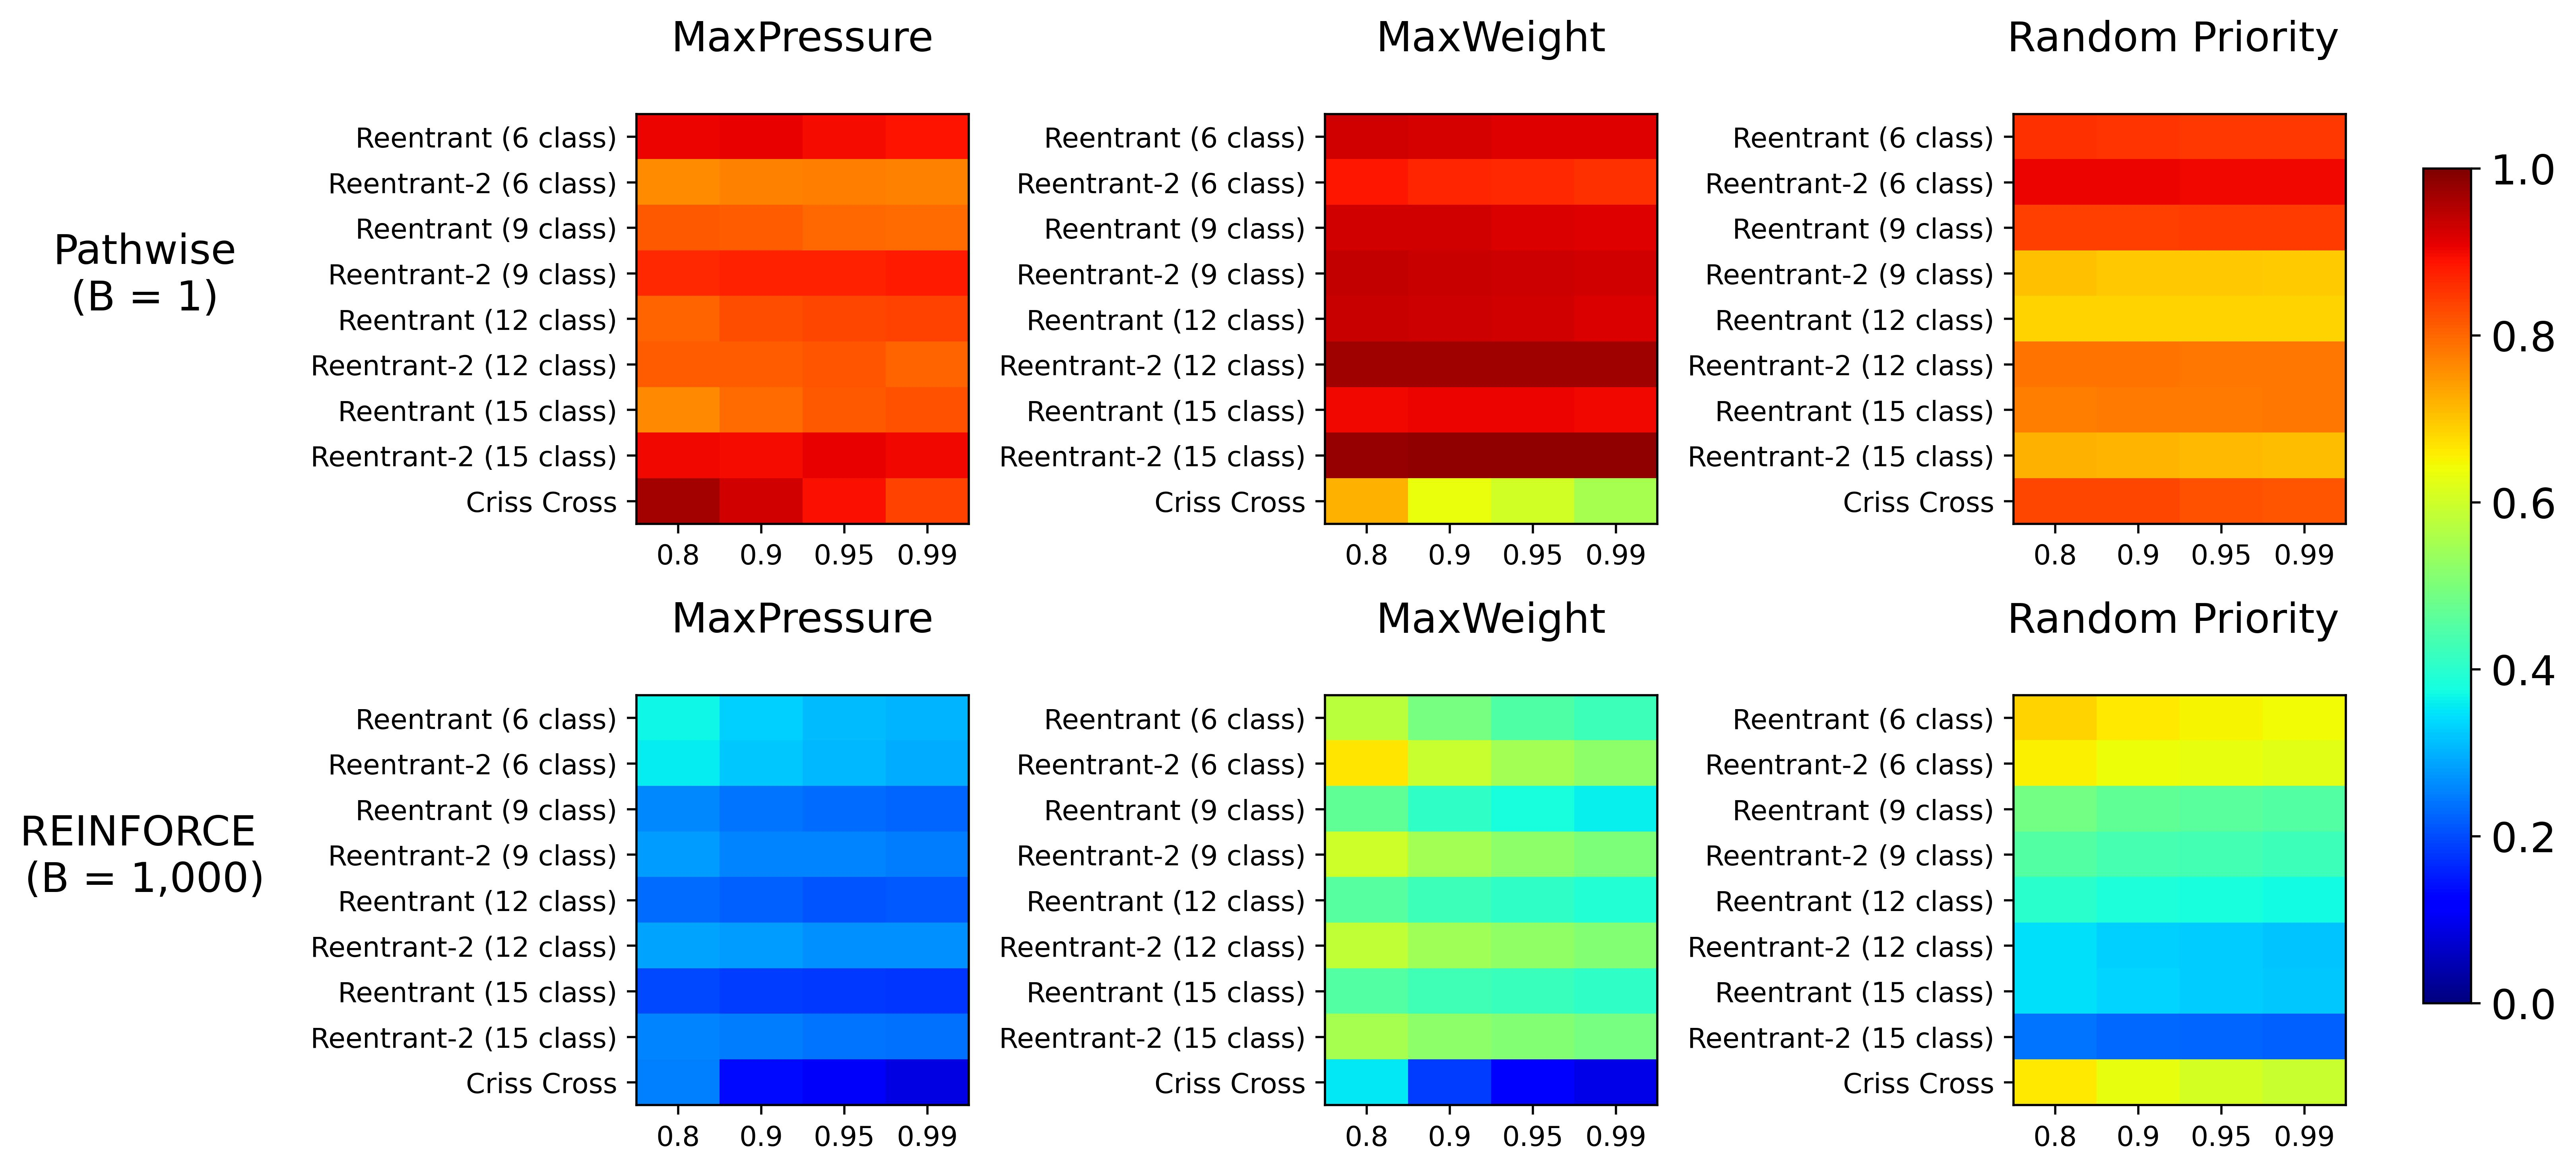
\includegraphics[height = 3.2in]{plot/gradient_eval/gradient_comparsion_policy.jpg}
    
    \caption{Comparison of estimation quality between $\pathwise$ and $\reinforce$ across several settings. We perform this comparison for 3 policies (soft MaxPressure, soft MaxWeight, soft Priority in~\eqref{eqn:soft_policies}), 9 network settings, and 4 levels of traffic intensity for each network. For each cell, we randomly draw $100$ parameters $\theta \in \R^{n}$. For each parameter, we estimate the true gradient by averaging the $\reinforce$ estimator over $10^{6}$ trajectories (with horizon $N = 1000$). We then compute the $\pathwise$ estimator with $B =1$ trajectory along with the $\reinforce$ estimator averaged across $B = 1000$ trajectories. In each instance, we draw 100 samples of these estimators to estimate $\cossim$, i.e., the average cosine similarity with the true gradient. In total, we perform this comparison across $10,800$ parameters. We find that across all of these diverse settings, $\pathwise$ delivers much higher fidelity to the true gradient, in many cases achieving an average cosine similarity close to the maximum value of 1, despite using orders of magnitude less data, whereas the cosine similarity of $\reinforce$ remains around $0.2$-$0.6$ even with 1000 trajectories.}
    \label{fig:gradient_comparison} 
\end{figure}

First, recall that a policy $\pi(x)$ maps queue-lengths $x$ to assignment between servers and queues, represented by an $m \times n$ matrix in $\overline{\mathcal{U}}$ (allowing for fractional routing matrices). We visit three classical queuing policies: priority policies~\cite{cox1961queues}, MaxWeight~\cite{tassiulas1990stability}, and MaxPressure~\cite{dai2005maximum}. Each of these methods selects the routing that solves an optimization problem. This means that the routing generated by the policy is deterministic given the state and is not differentiable in the policy parameters. In order to apply either $\reinforce$ or the $\pathwise$ gradient estimator to compute a policy gradient, we require differentiable surrogates of these policies. To this end, we define softened and parameterized variants of these policies, denoted as soft priority ($\mathsf{sPR}$), soft MaxWeight ($\mathsf{sMW}$), and soft MaxPressure ($\mathsf{sMP}$),
\begin{equation}
\label{eqn:soft_policies}
\pi^{\mathsf{sPR}}_{\theta}(x)_{i}= \softmax(\theta_{j} \cdot \mu_{i}), \quad
\pi^{\mathsf{sMW}}_{\theta}(x)_{i}= 
\softmax(\theta_{j}x_{j} \cdot \mu_{i}), \quad 
\pi^{\mathsf{sMP}}_{\theta}(x)_{i} = \softmax((\mu \odot R(\theta x))_{i})
\end{equation}
where $\theta \in \R_{+}^{n}$ are a vector of costs/weights for each queue, $\mu$ denotes the matrix of service rates with $\mu_{i} \in \R_{+}^{n}$ denoting the service rates associated with server $i$. 
The operation $\odot$ refers to element-wise multiplication and the
$\softmax$ operation maps a vector $a \in \R^{n}$ into a set of probabilities $\softmax(a)_{i} = e^{a_{i}} / \sum_{j=1}^{n} e^{a_{j}}$.






We are interested in identifying the parameter $\theta$ that minimizes long-run average holding cost where $c(x,u) = h^{\top} x$. 
%Note that when $\theta = h$, these correspond with the standard definitions of the above policies. 
We use the objective 
$J_{N}(\theta) = \E\left[\sum_{k=0}^{N-1}c(x_{k},\pi_{\theta}(x_{k}))\tau^{*}_{k+1}\right]$
where $N$ is a large enough number to approximate the long-run performance, and the goal of the gradient estimation is to estimate $\nabla J_{N}(\theta)$.

We consider the following environments, which appear throughout our computational experiments and serve as standard benchmarks for control policies in multi-class queuing networks. We describe the network structure in detail in Figure~\ref{fig:networks}.
\begin{itemize}
\item {\bf Criss-cross:} The network introduced in Example~\ref{example:criss-cross} (see Figure~\ref{fig:networks} (c)).
\item {\bf Re-entrant 1 ($n$ classes):} We consider a family of multi-class re-entrant networks with a varying number of classes, which was studied in~\cite{bertsimas2014robust,dai2022queueing}. The network is composed of several layers and each layer has 3 queues. Jobs processed in one layer are sent to the next layer. Arrivals to the system come to queues 1 and 3 in the first layer while queue 2 receives re-entered jobs from the last layer (see Figure~\ref{fig:networks} (a) for a two-layer example).
\item {\bf Re-entrant 2 ($n$ classes):} We consider another family of re-entrant network architecture that was studied in~\cite{bertsimas2014robust}. It also consists of multiple layers with 3 queues in each layer. It differs from the Re-entrant 1 environment in that only queue 1 receive external arrivals while queues 2 and 3 receive re-entered jobs from the last layer (see Figure~\ref{fig:networks} (b) for a two-layer example).
\end{itemize}

For a gradient estimator $\hat{g}$, the main performance metric we evaluate is $\cossim(\hat{g})$, which is the expected cosine similarity with the ground-truth gradient,
\begin{equation}
\label{eqn:similarity}
\cossim(\hat{g}) \equiv \E[\mathsf{cos} \left( \hat{g}, \nabla J_{N}(\theta) \right)] = \E \left[ \frac{ \langle \hat{g}, \nabla J_{N}(\theta) \rangle}{\norm{\hat{g}} \norm{ \nabla J_{N}(\theta)}} \right] \in [-1,1]
\end{equation}
where the expectation $\E$ is over randomness in $\hat{g}$. The higher the similarity is, the more aligned $\hat{g}$ is to the direction of $\nabla J_{N}(\theta)$. This metric incorporates both bias and variance of the gradient estimator. If the gradient estimator is unbiased but has a high variance, then each individual realization of $\hat{g}$ is likely to have low correlation with the true gradient, so the average cosine similarity will be small even if $\E[\hat{g}]=\nabla J_{N}(\theta)$. At the same time, if the gradient estimator has a low variance but a high bias, then the $\cossim(\hat{g})$ could still be small if $\mathsf{cos} \left(\E[\hat{g}], \nabla J_{N}(\theta) \right)$ is small. We focus on this metric, because it directly determines how informative the gradient estimates are when applying various gradient descent algorithms.  
For our experiments, we evaluate (a close approximation of) the ground-truth gradient $\nabla J_{N}(\theta)$
by using the unbiased $\reinforce$ gradient estimator over exceedingly many trajectories (in our case, $10^{6}$ trajectories). 

We compare the similarity of $\pathwise$ with that of $\reinforce$. 
%where $\reinforce$ is averaged over multiple trajectories. 
We denote $B$ as the number of trajectories we use to calculate each $\pathwise$ or $\reinforce$ gradient estimator.
\begin{align}
\underbrace{\hat{\nabla}_{\theta} J_{N}(\theta; \xi^{(1)}_{1:N})}_{\pathwise\text{ with }B=1} \qquad
\underbrace{\hat{\nabla}^{\mathsf{R}}_{\theta} J_{N,B}(\theta; \xi_{1:N}) := \frac{1}{B} \sum_{b = 1}^{B} \hat{\nabla}^{\mathsf{R}}_{\theta} J_{N}(\theta; \xi^{(b)}_{1:N})}_{\reinforce\text{ with }B\text{ trajectories}}
\end{align}
We compute the $\pathwise$ gradient with only $B = 1$ trajectory, while $\reinforce$ gradient is calculated using $B=10^3$ trajectories.
%to test the improvements in efficiency achieved by the estimator. 
For each policy and setting, we compute these gradients for $100$ different randomly generated values of $\theta$, which are drawn from a $\mathsf{Lognormal}(0,1)$ distribution (as the parameters must be positive in these policies). In total, we compare the gradients in $10,080$ unique parameter settings, and each gradient estimator is computed $100$ times to evaluate the average cosine similarity. When computing the policy gradient, we consider a time horizon of $N = 10^3$ steps. 
% \hntodo{This is great---you should repeat this in abstract, intro, and subsequent sections. This adds credibility.}
% {\color{blue} to approximate the long-run average cost?}.



Figure~\ref{fig:gradient_comparison} compares the $\pathwise$ estimator with $B = 1$ trajectory with the $\reinforce$ estimator averaged over $B = 10^3$ trajectories. For the $\reinforce$ estimator, costs are computed with a discount factor $\gamma = 0.999$, as using a lower discount rate introduced significant bias in the estimation. For $\pathwise$, we use an inverse temperature $\beta = 1$ for the $\softmin$ relaxation across all settings. 
% \hntodo{This part is uber important. See also my comments in the previous section. You need to say this at every section including the abstract, and really highlight that you did not tune this. It needs to come out that you chose $\beta = 1$ because it's a nice round number.} 
Each cell in Figure~\ref{fig:gradient_comparison} corresponds to a (policy, network, traffic-intensity) and the cell value is the average expected cosine similarity of the estimator averaged across the $100$ randomly drawn $\theta$ values. We observe that across these diverse settings, the $\pathwise$ estimator consistently has a much higher average cosine similarity with the true gradient despite using only a single trajectory. In fact, for {\bf 94.5\%} of the 10,800 parameter settings, $\pathwise$ has a higher average cosine similarity with 99\% confidence than $\reinforce$ with $B = 1000$ trajectories. In most cases, the cosine similarity of $\pathwise$ is close to 1, indicating almost perfect alignment with the true gradient even under high congestion. $\reinforce$ on the other hand suffers greatly from high variance. 
% We also observe in the left panel of Figure~\ref{fig:gradient_cossim_eval}, which displays the histogram of the similarity metric for each of the $10,080$ parameter settings, that this improvement in efficiency occurs across almost all parameter settings (with the exception of a few outliers). 
Overall, this demonstrates that $\pathwise$ is able to deliver greater estimation accuracy with an order of magnitude fewer samples.

% {\color{blue} talk about the dial plot}
% \begin{figure}[t]

% 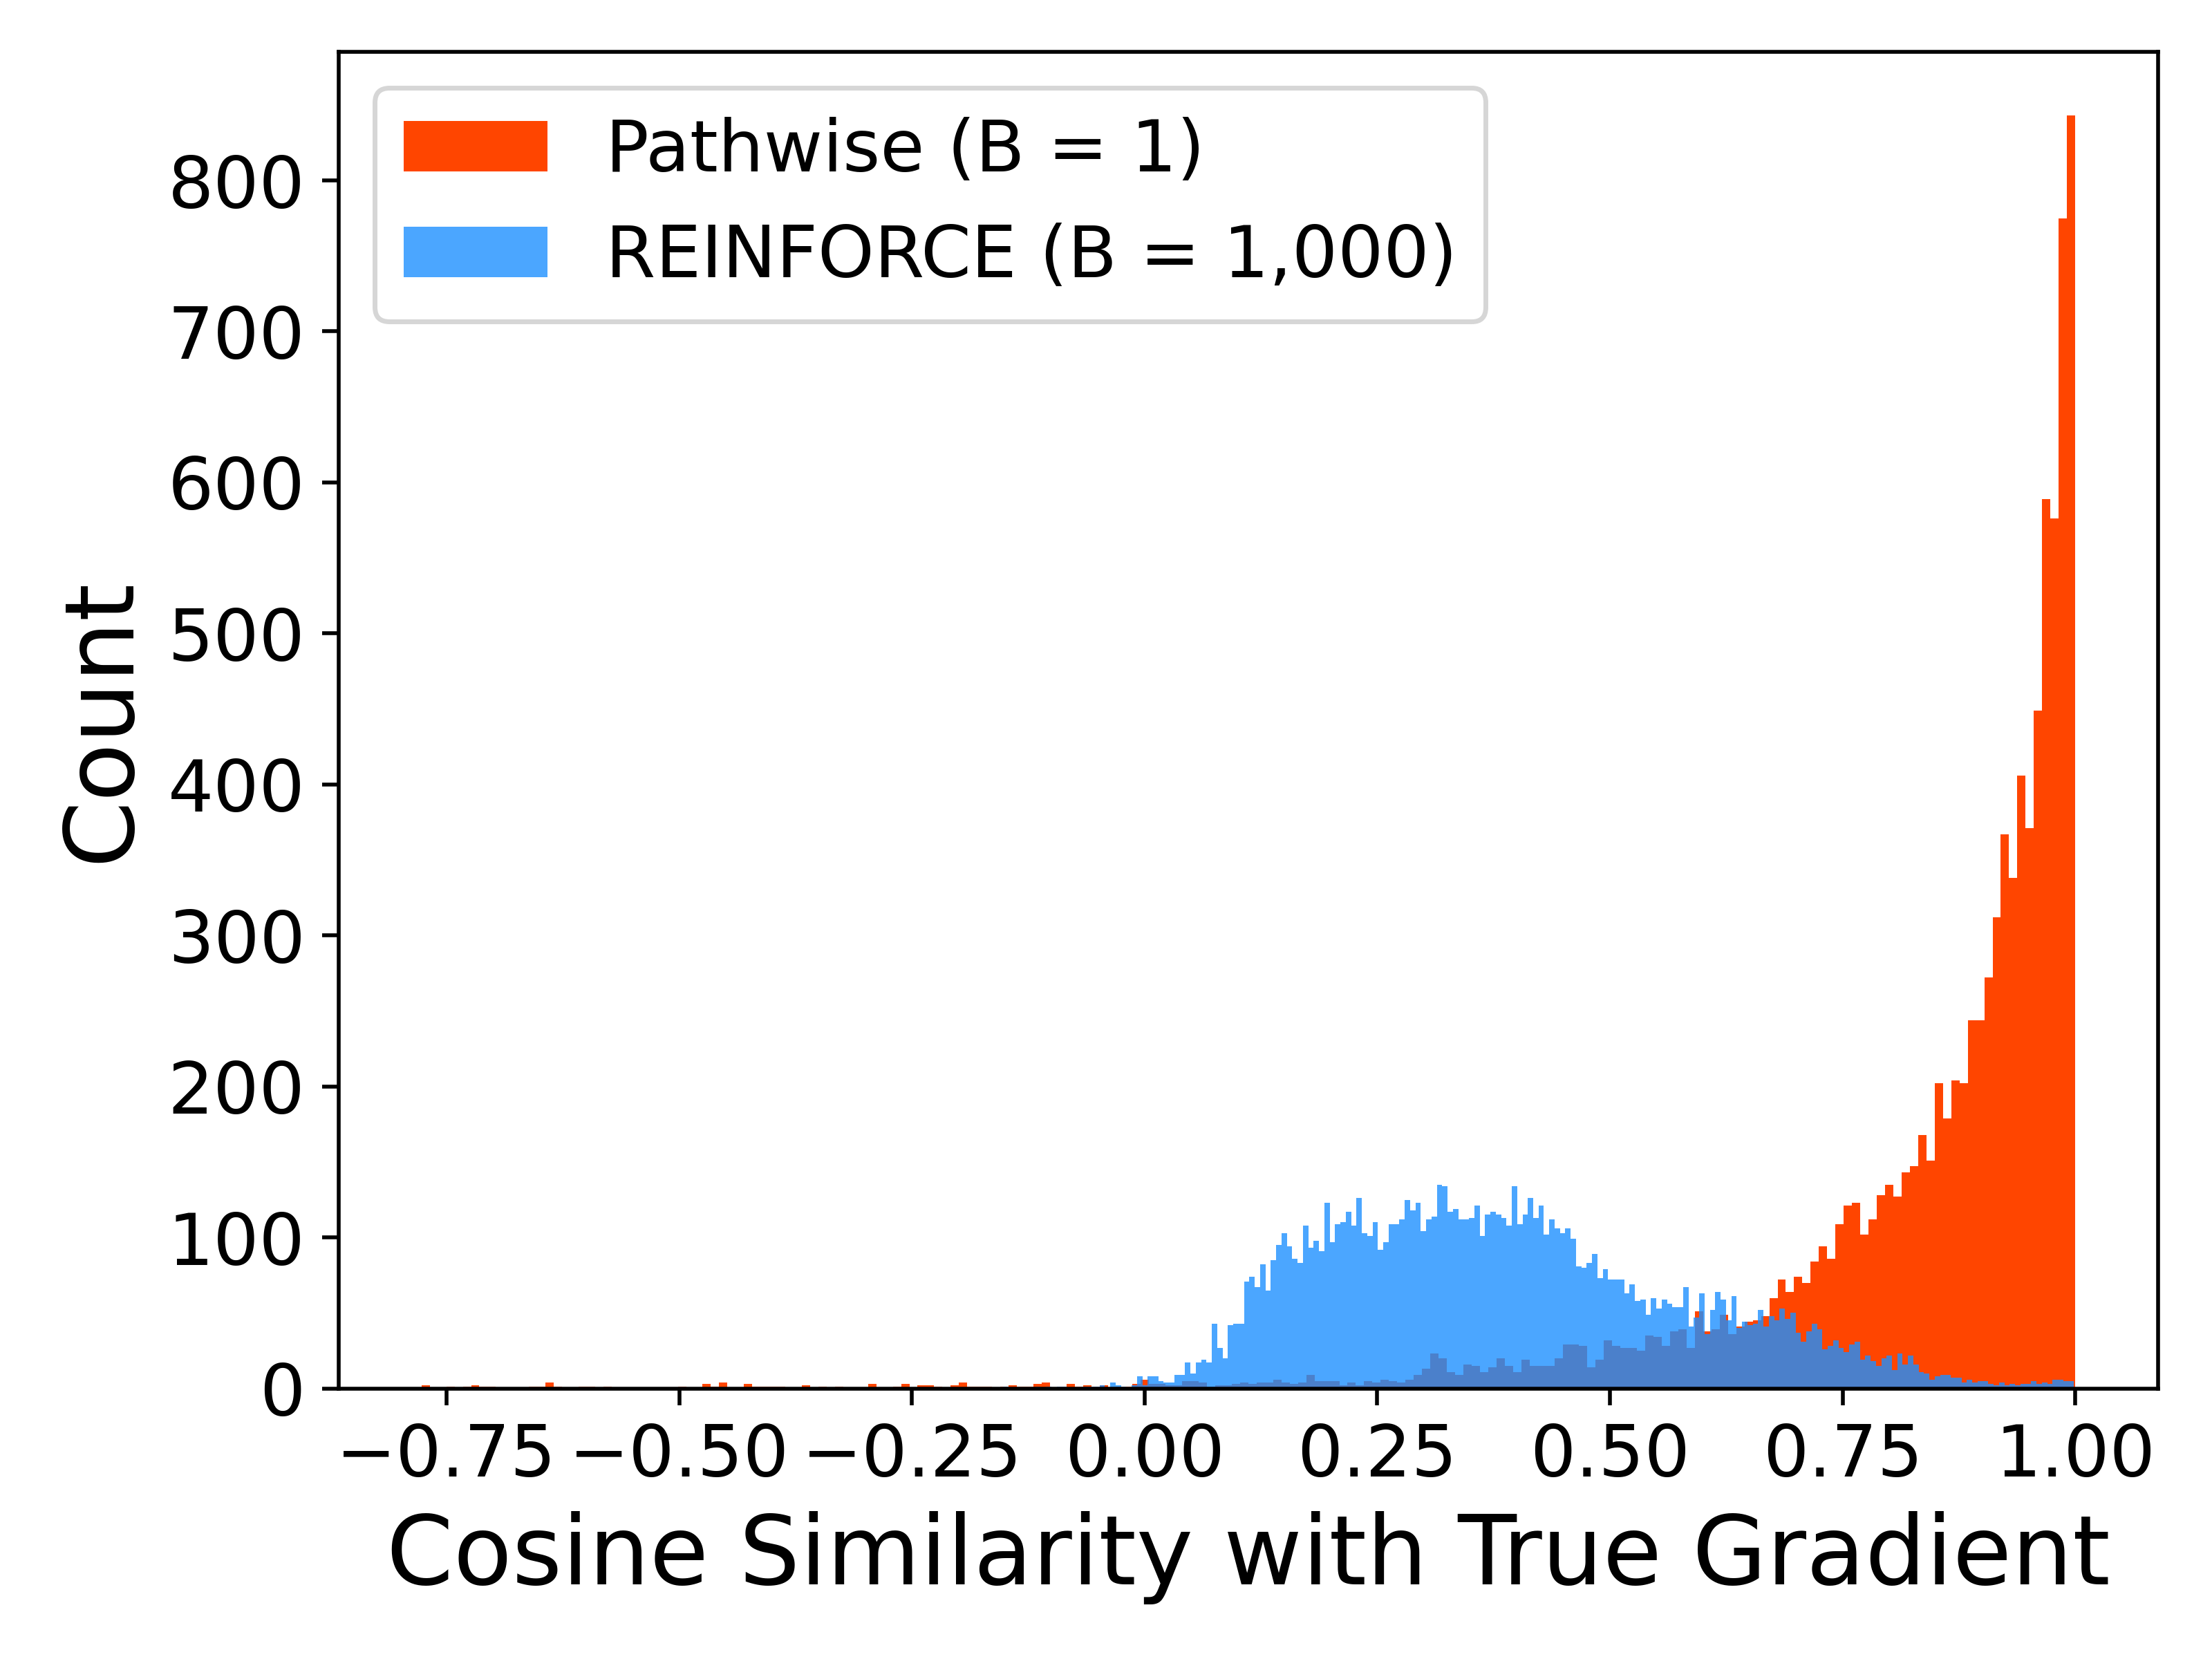
\includegraphics[height = 2.2in]{plot/gradient_eval/hist_cosine_sim.png}
% 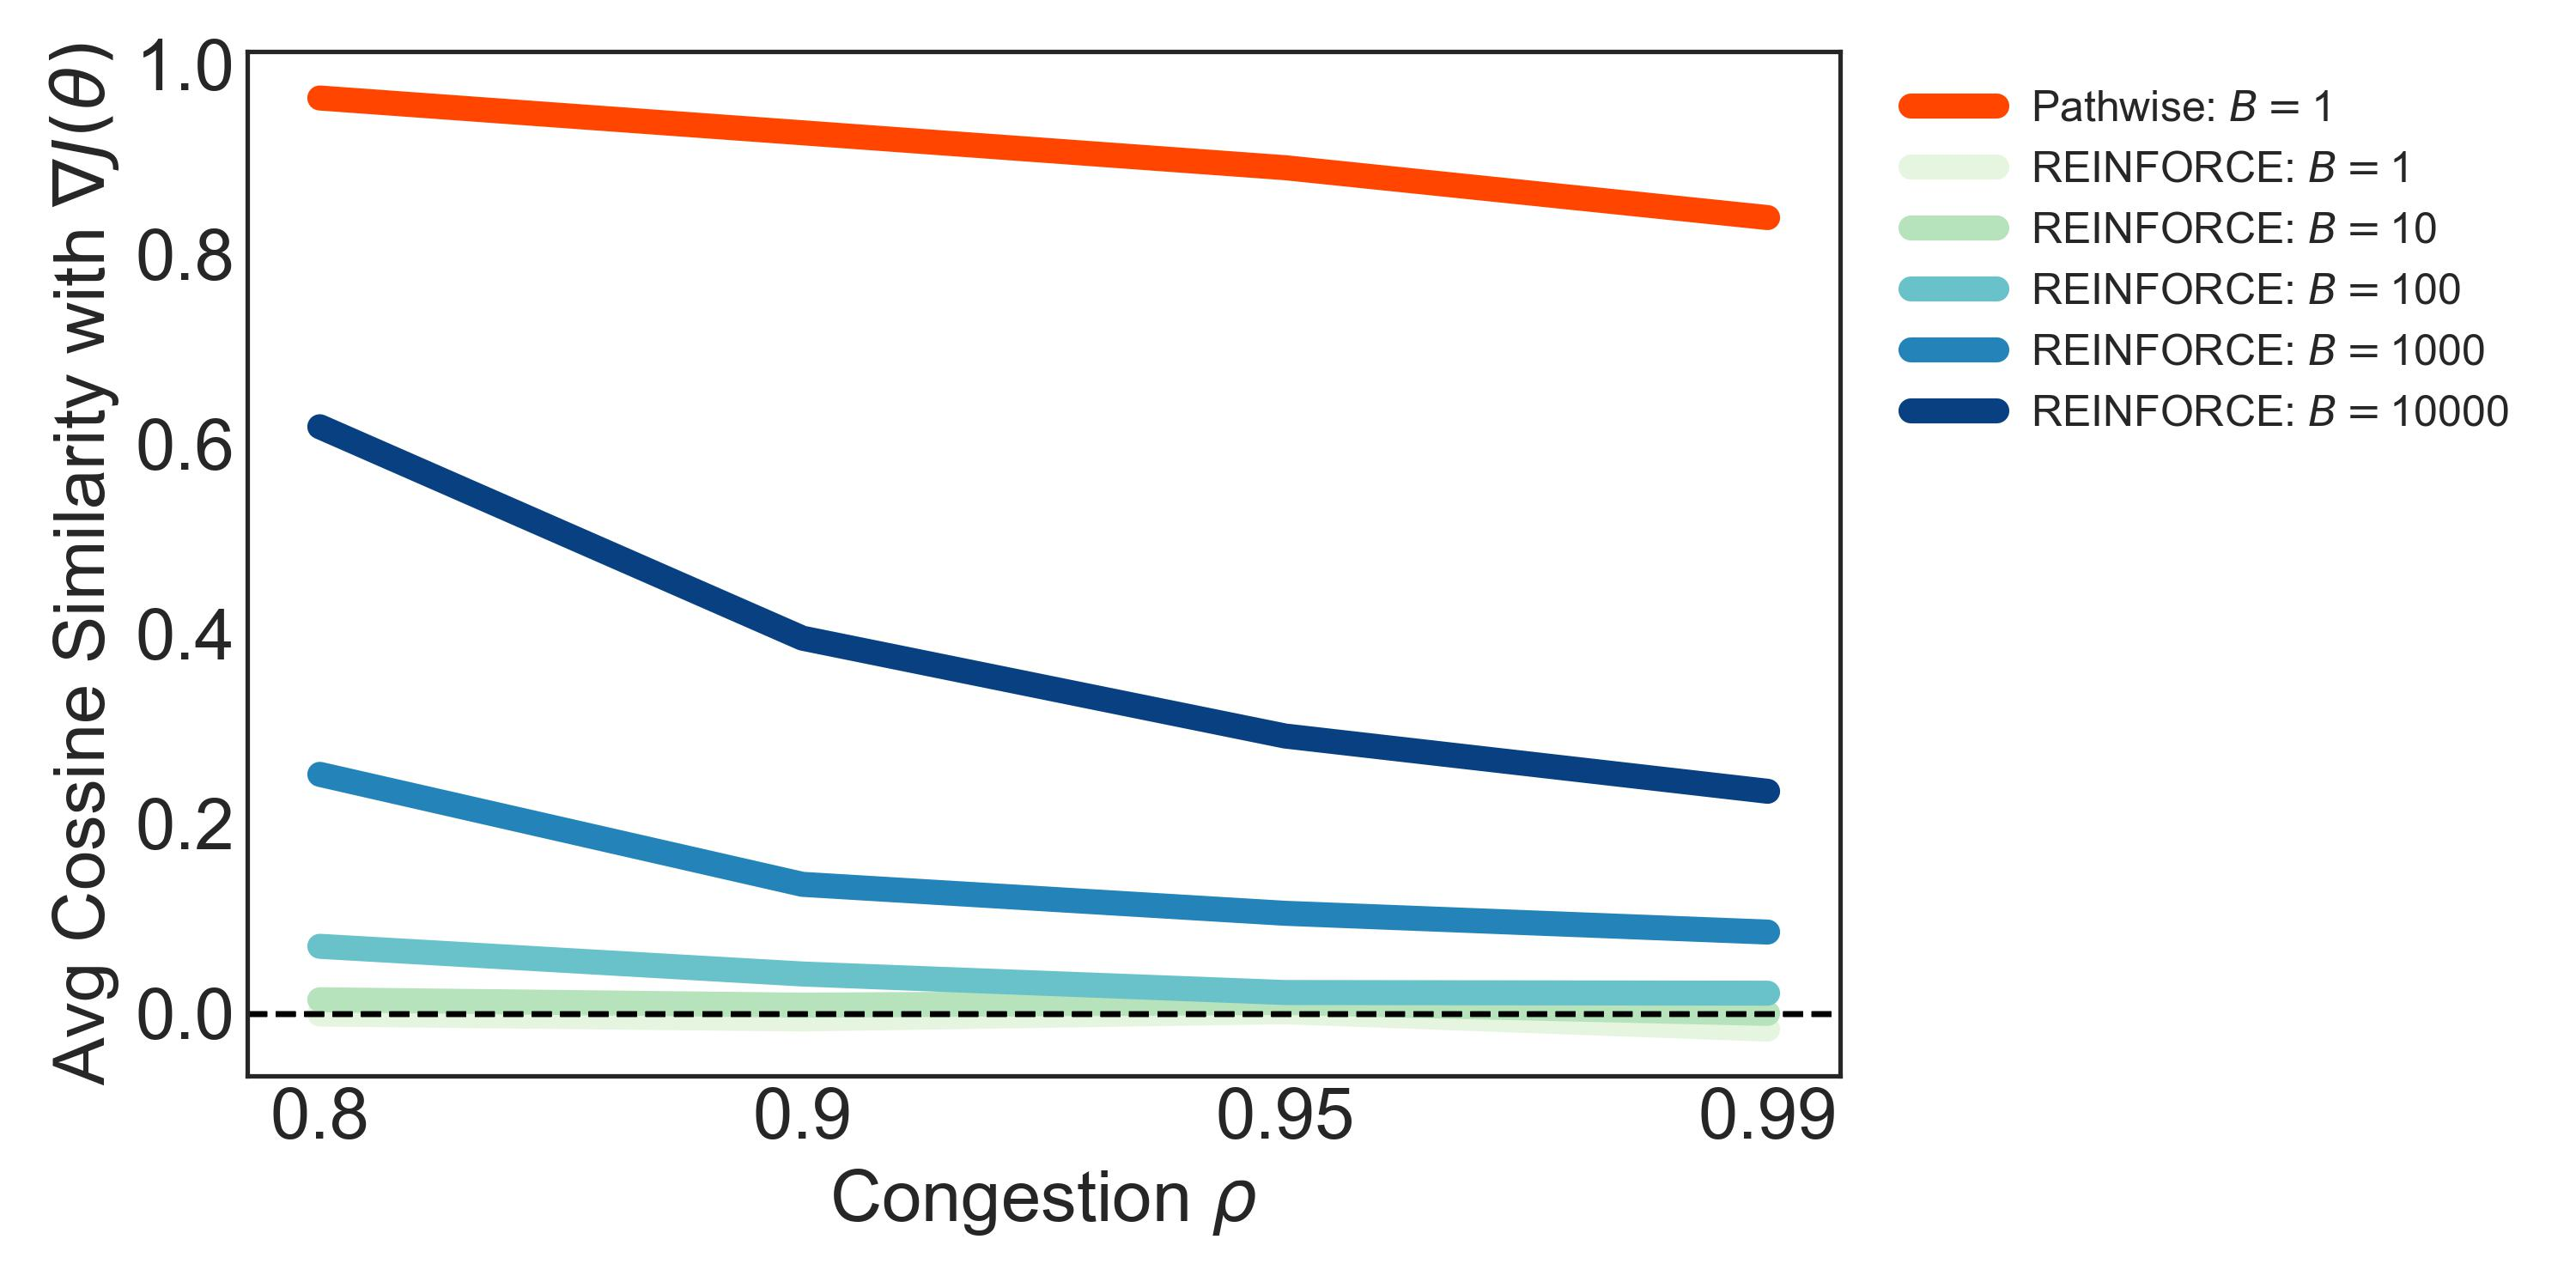
\includegraphics[height = 2.2in]{plot/gradient_eval/cossim_rho.jpg}
    
%     \caption{Cosine similarity of gradient estimators with the true gradient. (Left) Histogram of average cosine similarity for $\reinforce$ ($B = 1000$) and $\pathwise$ ($B = 1$) across $10,800$ parameter settings. $\pathwise$ consistently attains high cosine similarity close to the maximum value of 1. On the other hand, the average cosine similarity of the $\reinforce$ estimator is centered around $[0.25 , 0.5]$. (Right) Average cosine similarity with the true policy gradient for a parameterized max-pressure policy in the criss-cross network. This displays how average cosine similarity degrades with higher traffic intensity. While the cosine similarity of $\pathwise$ with only $B = 1$ trajectory degrades from $\approx 1$ to $\approx 0.8$, $\reinforce$ with $B = 10,000$ trajectories experiences a sharper degradation, from $0.6$ to $0.3$. $\reinforce$ with fewer trajectories does poorly across all traffic intensities.}
%     \label{fig:gradient_cossim_eval} 
% \end{figure}

% \subsection{Optimization tasks}

% Given the strong improvements in estimation efficiency, we now see how they translate to downstream optimization tasks.



\subsection{Learning the $c\mu$ rule}
\label{section:learn_cmu}
Given the strong improvements in estimation efficiency, we turn to evaluate how these translate to a downstream optimization task.
In single-server multi-class queues, it is well-known that the $c\mu$-rule minimizes the long-run average holding cost~\cite{cox1961queues}. We assess whether gradient descent with the $\reinforce$ or $\pathwise$ gradients is capable of converging to the $c\mu$-rule, without knowing the holding costs $h$ or $\mu$ and only using feedback from the environment. Despite its simplicity, it has been observed in prior work that this is a difficult learning task, particularly under heavy traffic~\cite{tran2022finding}.

We revisit the soft priority policy mentioned before, but with only the parameters $\theta\in \R^{n}$, i.e., 
\begin{equation}
\label{eq:soft_priority}
\pi^{\mathsf{sPR}}_{\theta}(x)_{i}= \softmax(\theta_{i})
\end{equation}
We also modify the policy to ensure that it is work-conserving, i.e., not assigning the server to an empty queue (see section~\ref{section:optimization} for further discussion).

We consider a family of multi-class single-server queues with $n$ queues. Holding costs are identically $h_{j} = 1$. Inter-arrival and service times are exponentially distributed, the service rates are $\mu_{1j} = 1 + \epsilon j$, for some $\epsilon>0$, and the arrival rates are identical $\lambda_{j} = \lambda$ and $\lambda$ are set such that the traffic intensity $\sum_{j=1}^{n} \frac{\lambda}{\mu_{1j}} = \rho$
%for $\rho = 0.95$
for some $\rho \in (0,1)$. Note that in this case, the $c\mu$-rule prioritizes queues with higher indices $j$. We consider a grid of gap sizes $\epsilon \in \{1.0, 0.5, 0.1, 0.05, 0.01 \}$ to adjust the difficulty of the problem; the smaller $\epsilon$ is, the harder it is to learn.

We compare $\pathwise$ with $B=1$ trajectory and $\reinforce$ with $B = 100$ trajectories for trajectories of $N = 1000$ steps. In order to isolate the effect of the gradient estimator from the optimization scheme, for both estimators we use an identical stochastic gradient descent scheme with normalized gradients (as these two estimators may differ by a scale factor). That is, for gradient estimator $\hat{g}$, the update under step-size $\alpha$ is
\[
\theta_{t+1} = \theta_{t} - \alpha \frac{\hat{g}}{\norm{\hat{g}}}.
\]
We run $T$ gradient descent steps for each gradient estimator. To allow for the fact that different estimators may have different performances across different step sizes, we consider a grid of step sizes $\alpha \in \{0.01, 0.1, 0.5, 1.0 \}$. Gradient normalization may prevent convergence, so we use the averaged iterate $\bar{\theta}_{T}$ for $T$. We then evaluate the long-run average holding cost under a strict priority policy determined by $\bar{\theta}_{T}$, i.e., $\pi_{\bar{\theta}_{T}}(x)_{i} = \argmax \bar{\theta}_{T,j}$. 
%to compare with the $c \mu$ rule.

% \begin{figure}[t]
% \centering

% 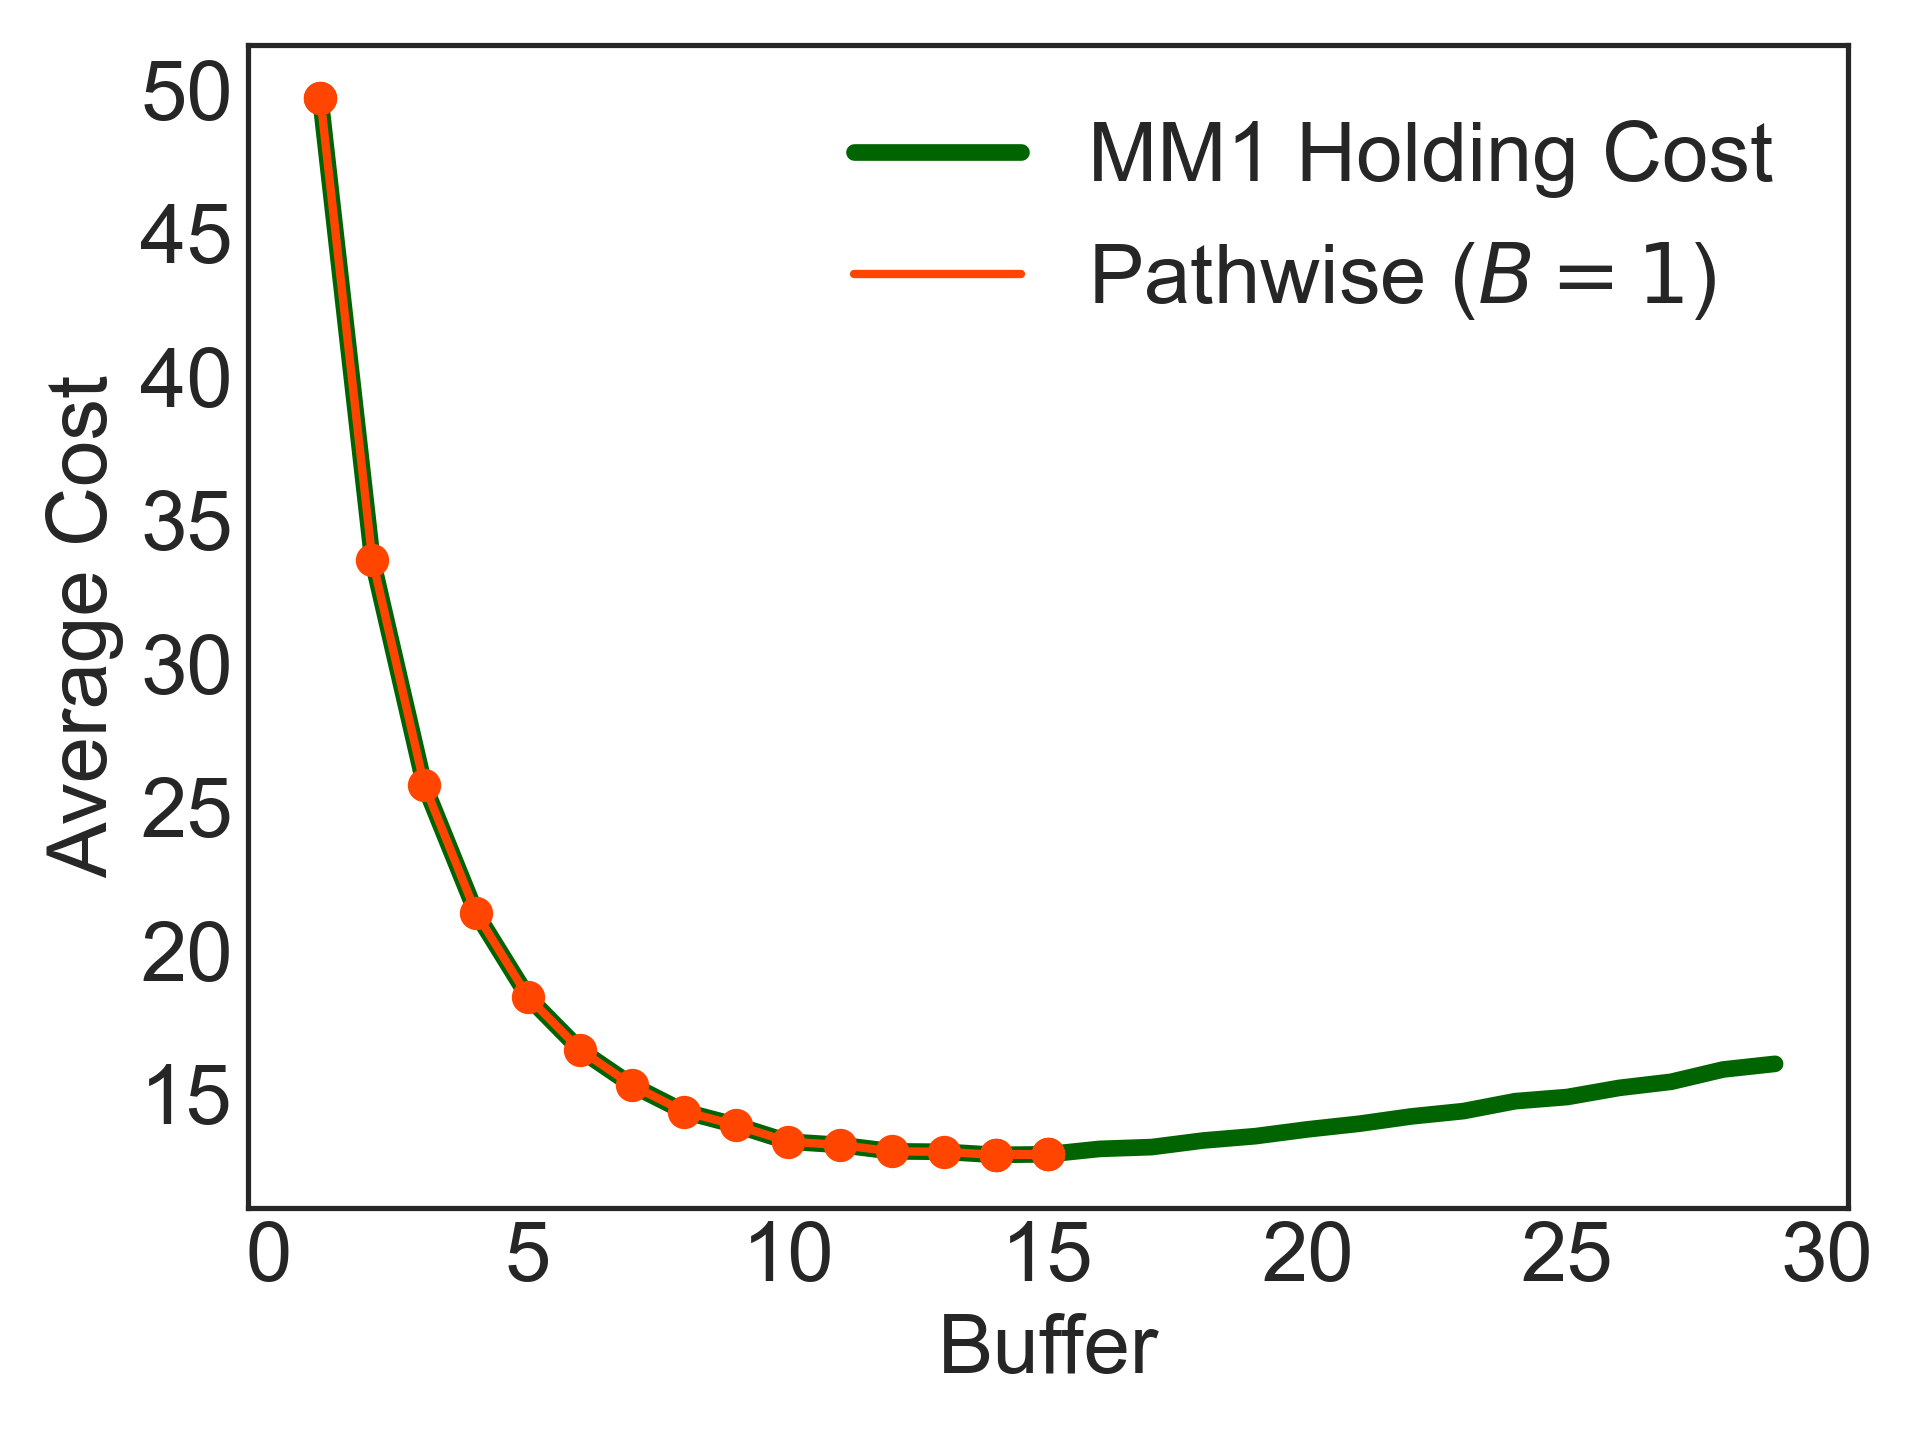
\includegraphics[height = 2.3in]{plot/gradient_eval/mm1_buffer_control_sgn.png}

    
%     \caption{Admission control.}
%     \label{fig:admission} 
% \end{figure}

\begin{figure}[t]
\centering
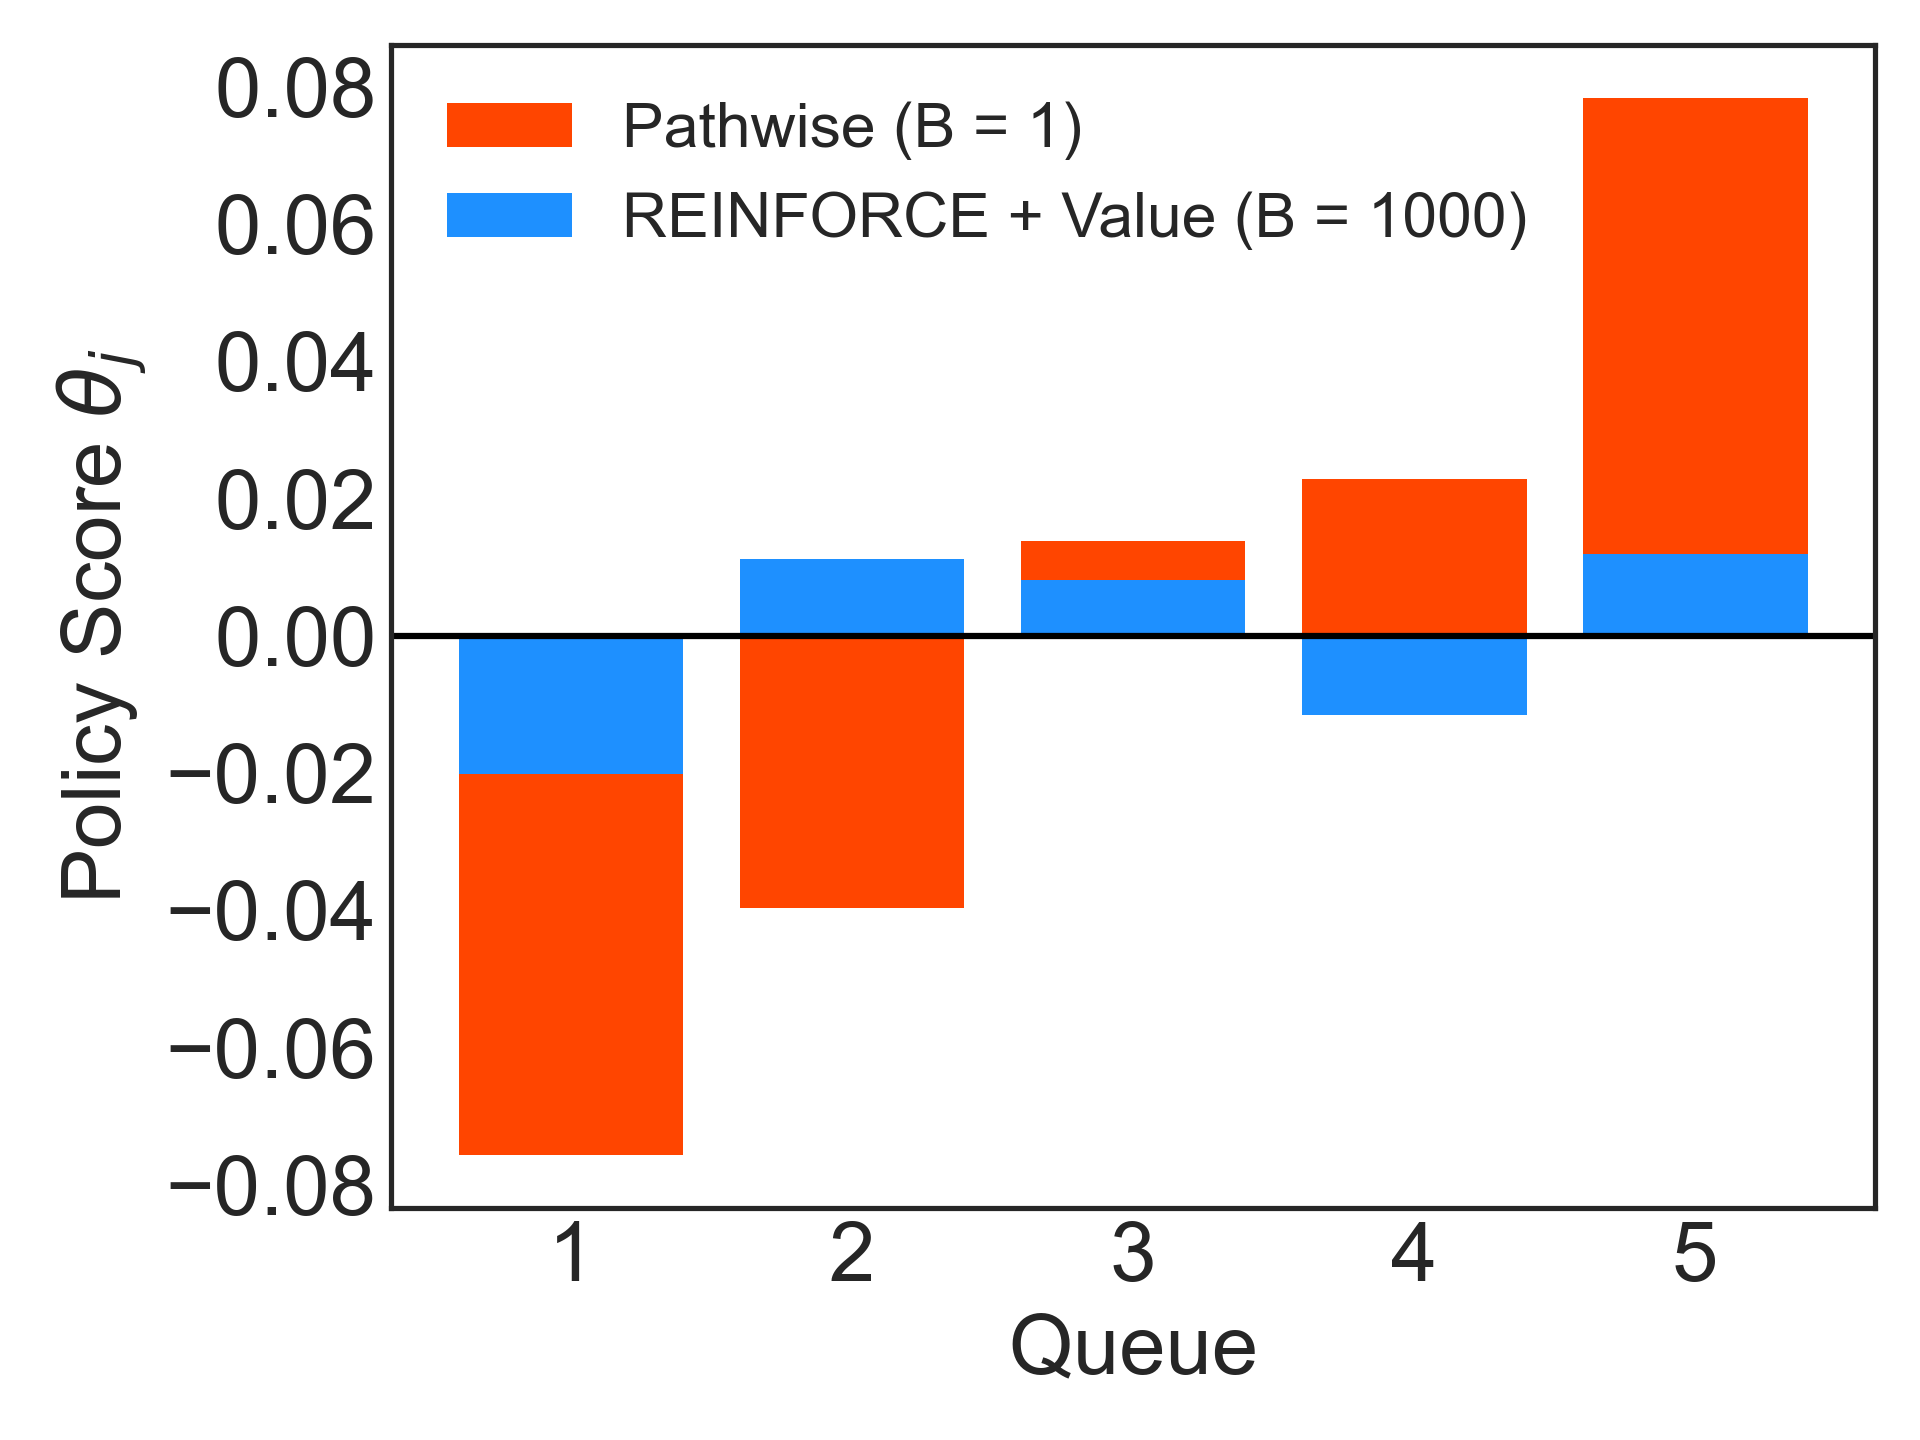
\includegraphics[height = 2.1in]{plot/gradient_eval/cmu_bar_q_5_value.png}
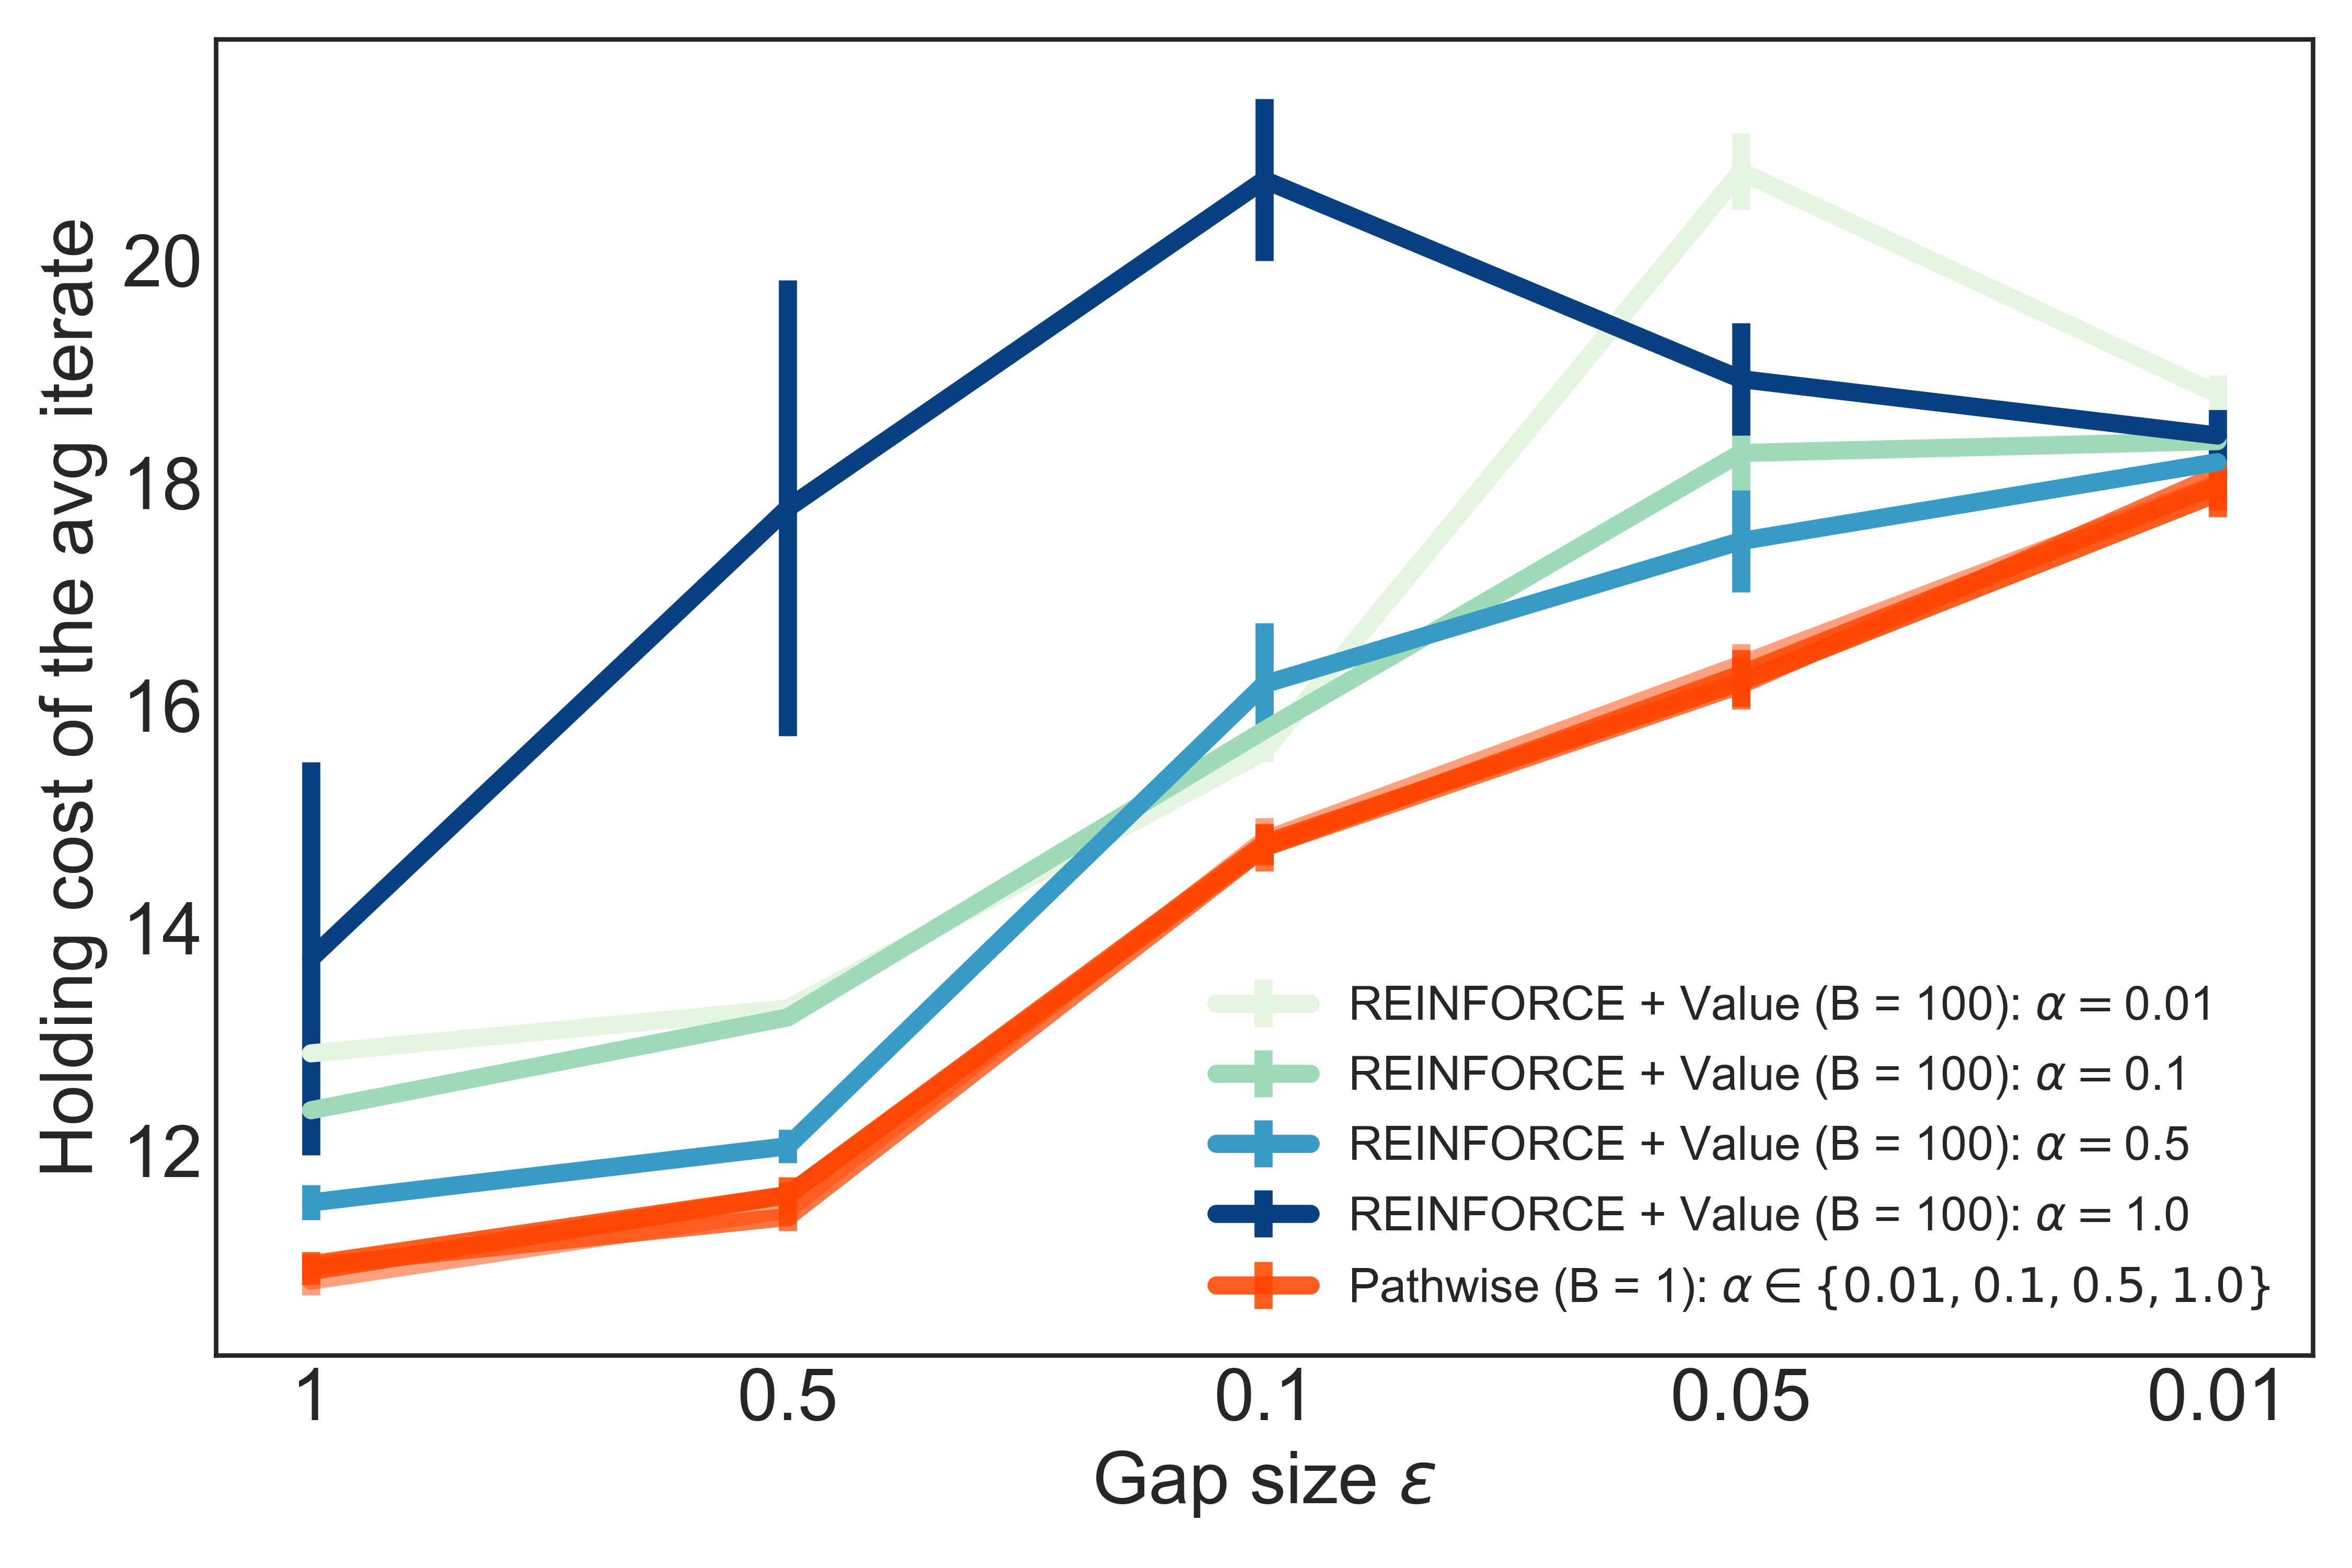
\includegraphics[height = 2.1in]{plot/gradient_eval/cmu_value_convergence.jpg}
    
    \caption{Learning the $c\mu$ rule. (Left) Averaged iterate of the policy parameters after 50 gradient steps with $\pathwise$ ($B = 1$) and $\reinforce$ ($B = 100$) gradients for a 5-class queue with traffic intensity $\rho = 0.99$ and gap-size $\epsilon = 0.1$. The scores obtained by $\pathwise$ are increasing in the queue index, which matches the ordering of the $c\mu$ index in this instance. The scores obtained by $\reinforce$ do not achieve the correct ordering despite using more trajectories. (Right) Average holding cost of the average iterate after 20 steps of gradient descent in a 10-class queue with $\rho = 0.95$. This figure reports the results averaged over 50 separate runs of gradient descent, across a grid of step-sizes (denoted as $\alpha$). Remarkably, the optimization performance of the $\pathwise$ estimator is highly similar across step-sizes, and \emph{uniformly} outperforms $\reinforce$ with different step-sizes $\alpha$. 
    %The improvement is higher in more difficult settings (corresponding to a smaller $\epsilon$), although for very small $\epsilon$ both methods have trouble learning the $c\mu$-rule.
    % {\color{blue} zoom into the orange line to see that it does the same across all step sizes}
    }
    \label{fig:cmu} 
\end{figure}

% {\color{blue} mention that pathwise the performance is basically the same across all step-sizes}

The left panel of Figure~\ref{fig:cmu} displays the values of $\bar{\theta}_{T}$ after $T=50$ gradient iterates for $\pathwise$ and $\reinforce$ with $n=5$, $\epsilon = 0.1$, and $\rho = 0.99$. We observe that while $\pathwise$ sorts the queues in the correct order (it should be increasing with the queue index), $\reinforce$ even with $B = 100$ trajectories fails to prioritize queues with a higher $c \mu$ index. Remarkably, we observe in the right panel of the same figure that $\pathwise$ with just a single trajectory achieves a lower average holding cost than $\reinforce$ {\bf uniformly} across various step sizes and difficulty levels, whereas the performance of $\reinforce$ varies greatly depending on the step size. This indicates that the improvements in gradient efficiency/accuracy of $\pathwise$ make it more robust to the step-size hyper-parameter. 
It is also worth mentioning that when gap size $\epsilon$ becomes smaller, it is more difficult to learn. At the same time, since $\mu_{1j}$'s are more similar to each other, the cost difference between different priority rules also diminishes.
%It is worth mentioning that while the cost reduction from $\pathwise$ is significant for most gap sizes $\epsilon$, for very small $\epsilon$ it becomes difficult to either method to identify the queue with the highest index, and the performance benefits from doing so also diminish.


% {\color{blue} mention that performance is the same for all $\epsilon$ because the problem gets too hard. and practically theres no difference}

\subsection{Admission Control}
\label{section:admission}

While we focus mainly on scheduling tasks in this work, our gradient estimation framework can also be applied to admission control, which is another fundamental queuing control task~\cite{naor1969regulation, chr1972individual, ccil2009effects, ghosh2007optimal, koccauga2010admission}. To manage congestion, the queuing network may reject new arrivals to the network if the queue lengths are above certain thresholds. The admission or buffer control problem is to select these thresholds to balance the trade-off between managing congestion and ensuring sufficient resource utilization.

Under fixed buffer sizes $\buff = \{\buff_{j}\}_{j=1}^{n}$, new arrivals to queue $j$ are blocked if $x_{j} = \buff_{j}$. As a result, the state update is modified as follows,
\begin{equation}
x_{k+1} = \min\{x_{k} + De_{k+1}, \buff\}.
\end{equation}
% \hntodo{Let's not use $\beta$ for the buffer; overlaps with the inverse temp. }
While a small $\buff$ can greatly reduce congestion, it can impede the system throughput. To account for this, we introduce a cost for rejecting an arrival to the network. Let $o_{k} \in \{0,1\}^{n}$ denote whether an arrival is \emph{overflowed}, i.e., an arrival is blocked because the buffer is full,
\begin{equation}
o_{k+1} = De_{k+1} \cdot 1\{
x_{k} + De_{k+1} > \buff \}.
\end{equation}
Given a fixed routing policy, the control task is to choose the buffer sizes $\buff$ to minimize the holding and overflow costs:
\begin{align}
%c(x, \buff) &= h^{\top}x + b^{\top}z \\
J_{N}(\buff;\xi_{1:N}) &=  \sum_{k=0}^{N-1}  (h^{\top}x_{k})\tau_{k+1}^{*} + b^{\top}o_{k}.
\end{align}
Similar to the routing control problem, despite the fact that overflow is discrete, our gradient estimation framework is capable of computing a $\pathwise$ gradient of the cost with respect to the buffer sizes, which we denote as $\widehat{\nabla}_{\buff} J_{N}(\buff;\xi_{1:N})$, i.e., we can evaluate gradients at integral values of the buffer size and use this to perform updates. Since the buffer sizes must be integral, 
%and Using the $\pathwise$ gradient $\widehat{\nabla}_{\buff} J_{N}(\buff;\xi_{1:N})$, 
we update the buffer sizes via sign gradient descent to preserve integrality:
\begin{equation}
\label{eq:sign_gd}
\buff_{t+1} = \buff_{t} - \mathsf{sign} \left( \widehat{\nabla}_{\buff} J_{N}(\buff;\xi_{1:N}) \right).
\end{equation}
% One could also optimize over purely integral values through sign gradient descent, but this achieves worse performance 
% \hntodo{In Figure~\ref{fig:admission}, explicitly write SGD stepsize instead of $\alpha$}

\begin{figure}[t]
\centering
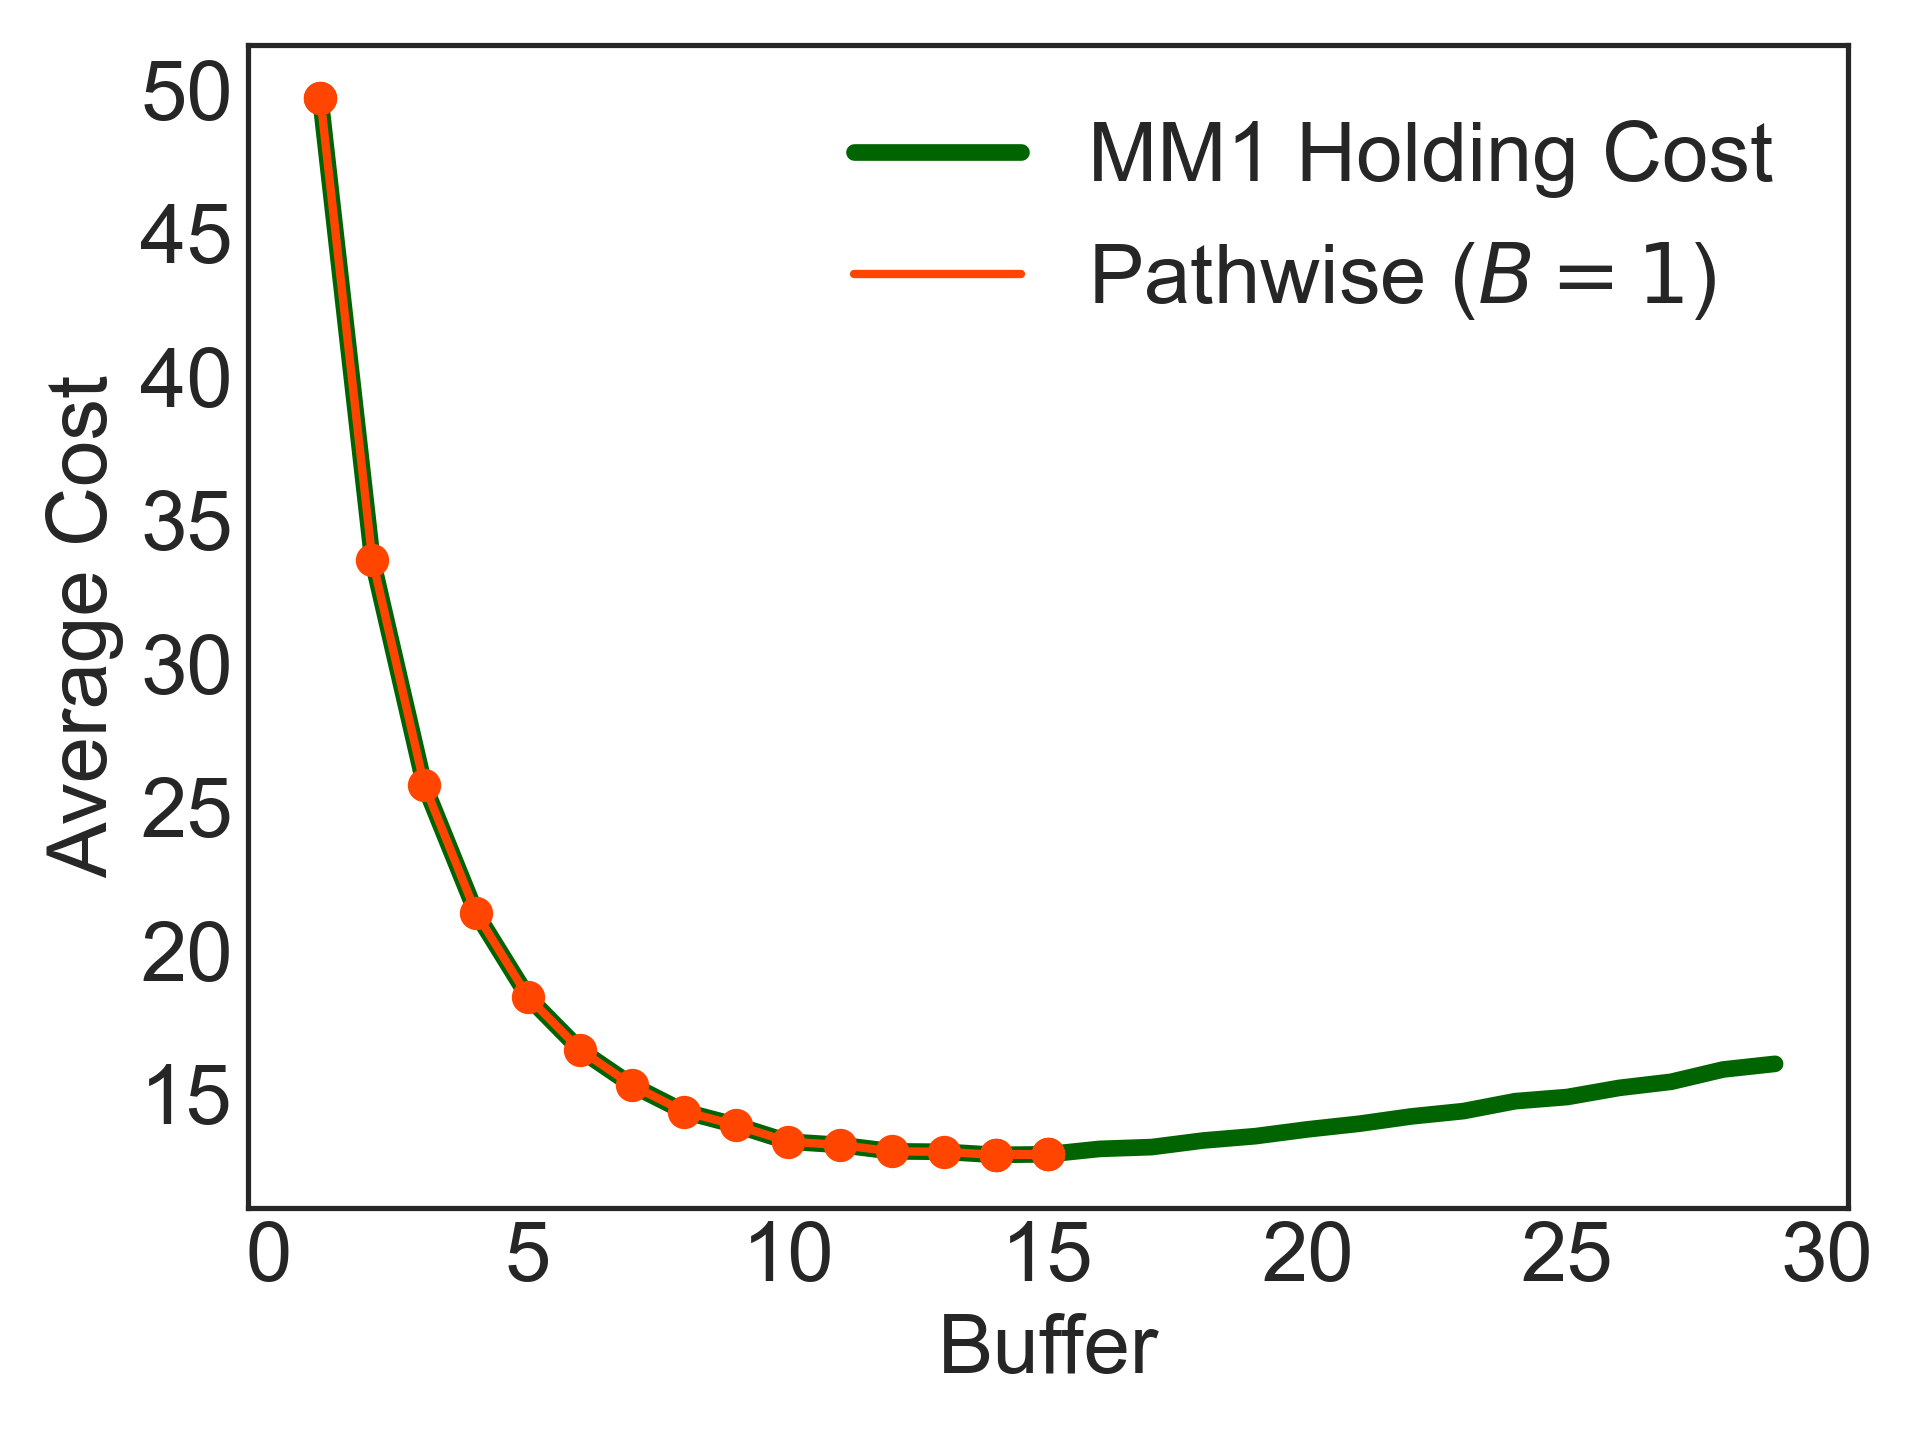
\includegraphics[height = 2.3in]{plot/gradient_eval/mm1_buffer_control_sgn.png}
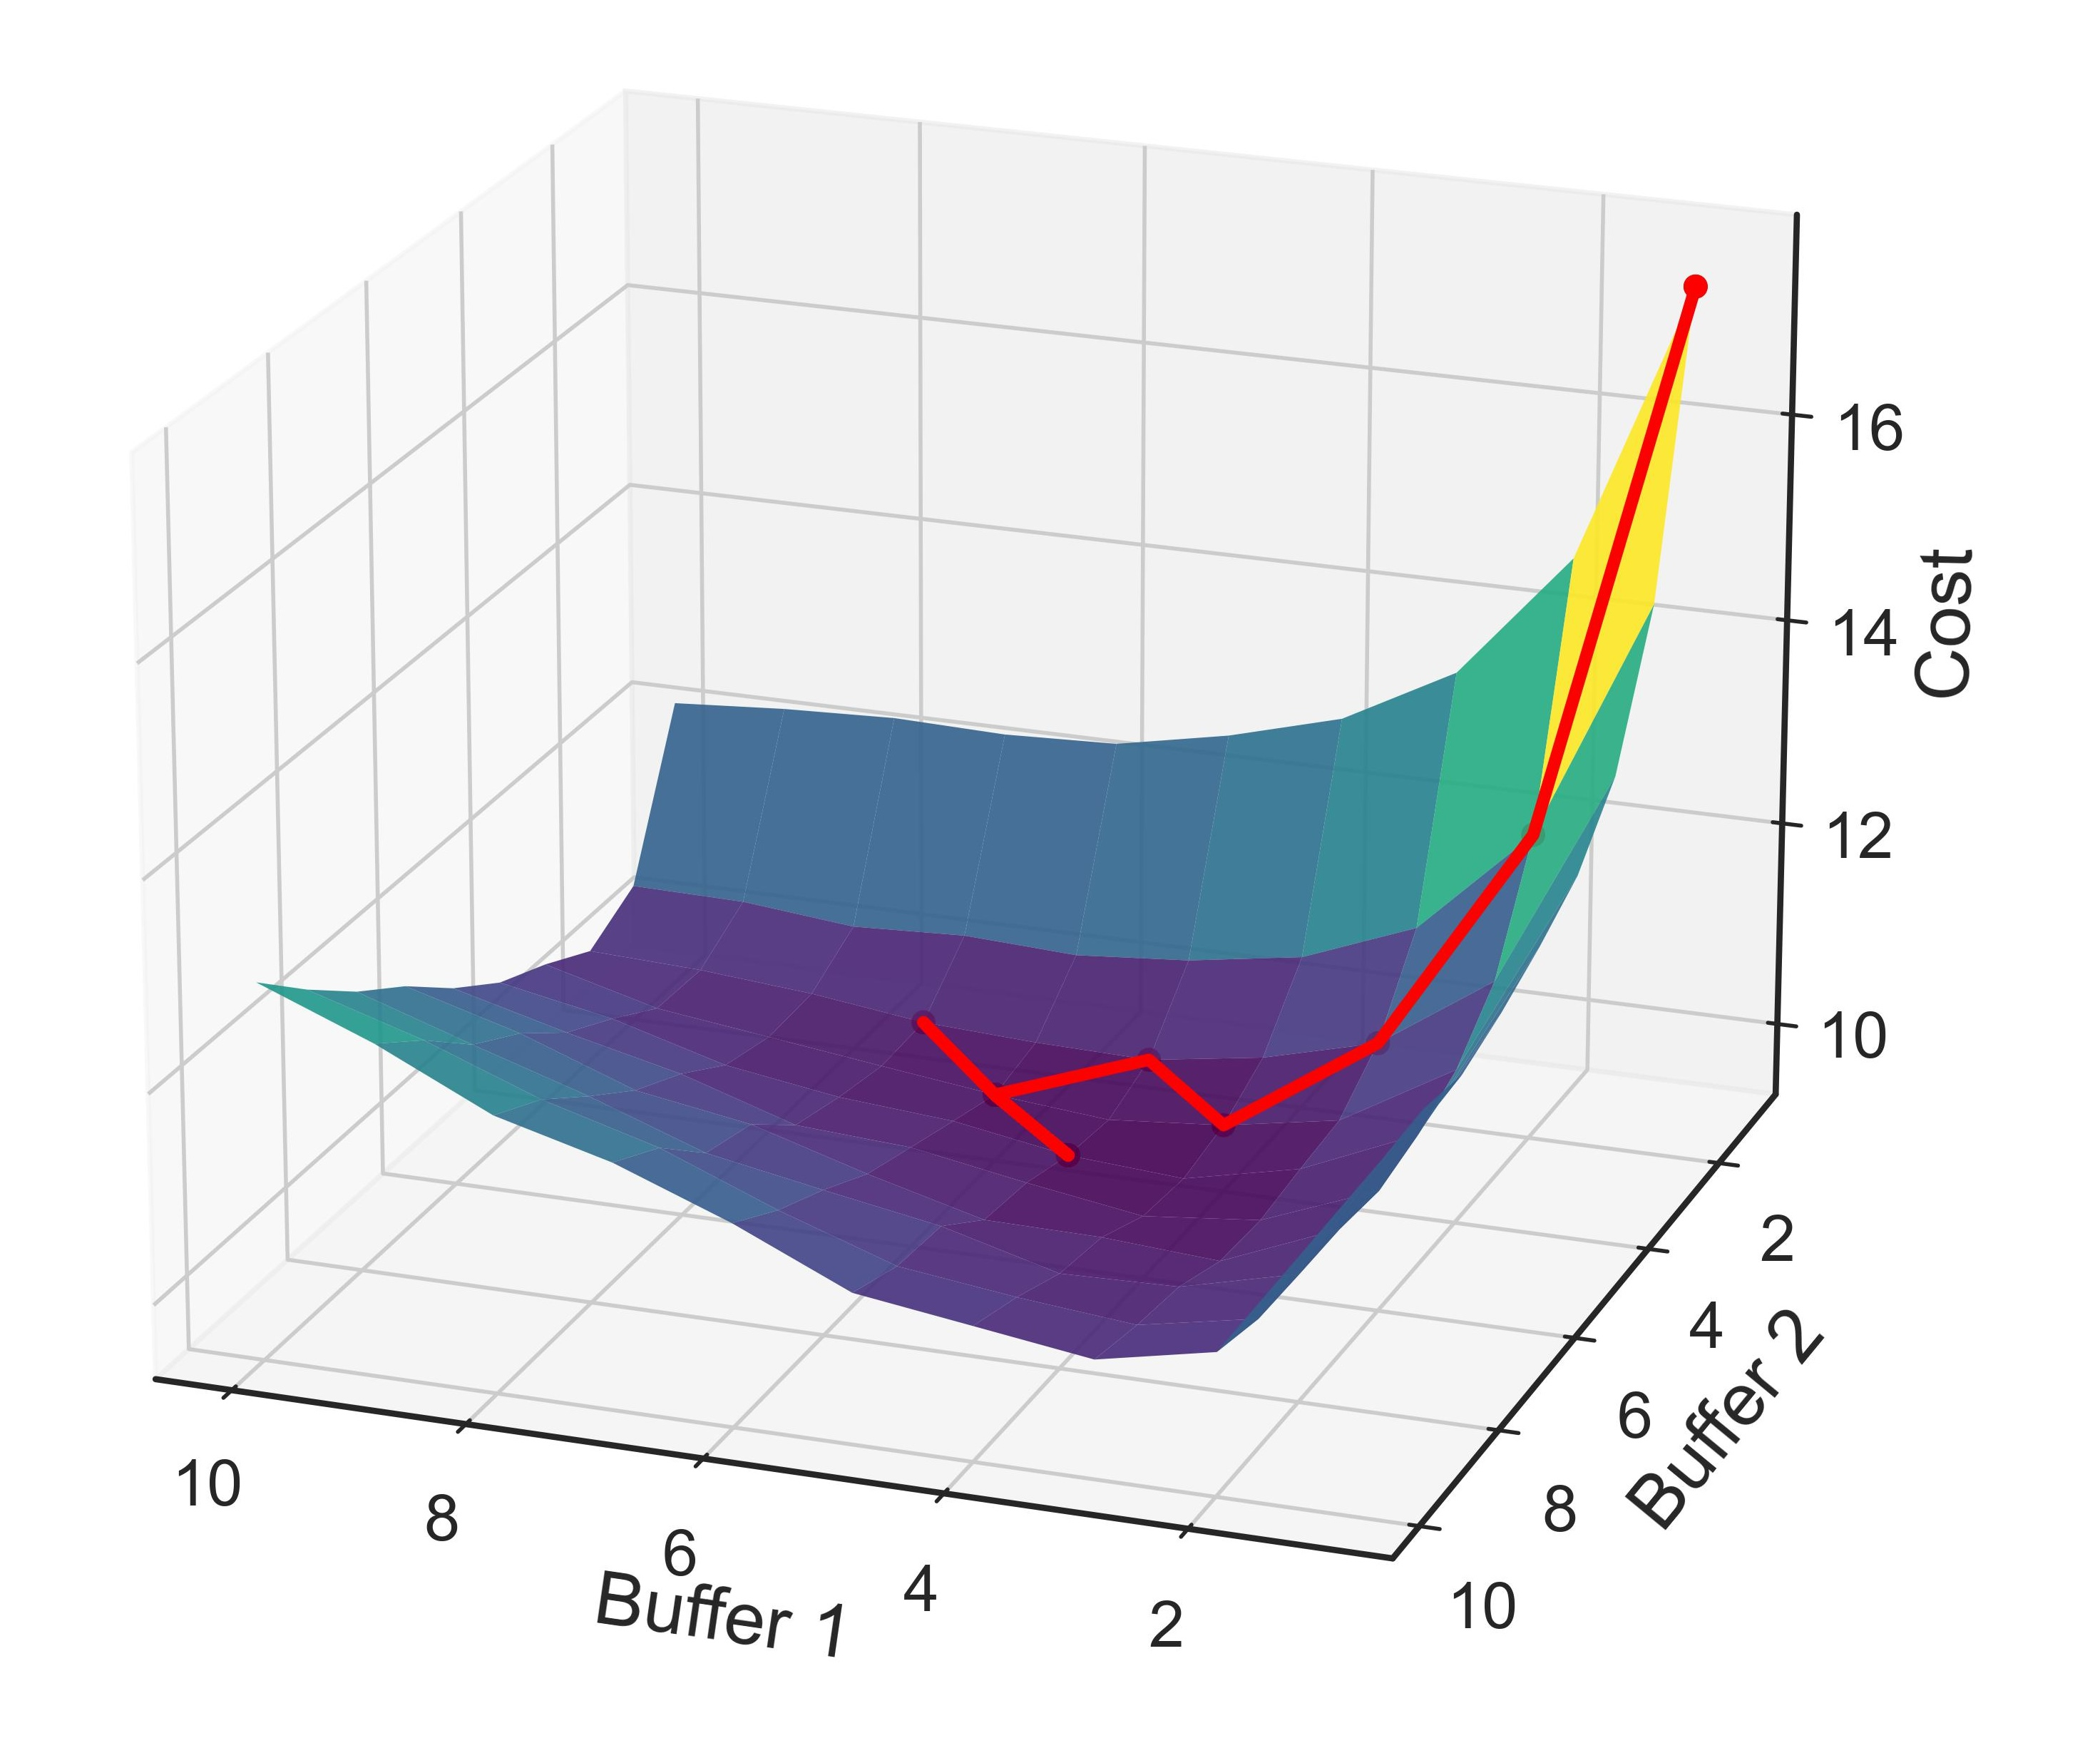
\includegraphics[height = 2.5in]{plot/gradient_eval/multiclass_admission_control.jpg}
    
    \caption{Gradient descent with $\pathwise$ for admission control tasks. (Left) Iterates of sign gradient descent with the $\pathwise$ estimator for the buffer size of an $M/M/1$ queue with holding cost $h = 1$ and overflow cost $b = 100$. Starting from $L_{0} = 1$, the iterates quickly converge to the optimal level of $L^{*} = 14$. (Right) buffer sizes obtained by sign gradient descent with the $\pathwise$ estimator for a 2 queue 1 server network with holding cost $h = 1$ and overflow cost $b = 20$. Starting from $L_{0} = (1,1)$, the iterates quickly converge to the basin of the loss surface. }
    \label{fig:admission} 
\end{figure}

Learning for admission control has been studied in the queuing and simulation literature~\cite{cassandras2002perturbation, cassandras2003perturbation, ho1983new, cohen2024learning}. While exact gradient methods are possible in fluid models~\cite{cassandras2002perturbation, cassandras2003perturbation}, the standard approach for discrete queuing models is finite perturbation analysis~\cite{ho1983new}, given the discrete nature of the buffer sizes.
Randomized finite-differences, which is also known as Simultaneous Perturbation Stochastic Approximation (SPSA)~\cite{spall1992multivariate, fu1997optimization}, is a popular optimization method for discrete search problems. This method forms a finite-differences gradient through a random perturbation. Let $\eta \sim \mathsf{Rademacher}(n, 1/2) \in \{-1,1 \}^{n}$ be a random $n$-dimensional vector where each component is an independent $\mathsf{Rademacher}$ random variable, taking values in $\{-1,1 \}$ with equal probability. For each perturbation $\eta$, we evaluate the objective at $\buff \pm \eta$, i.e., $J_N(\buff + \eta; \xi_{1:N})$ and $J_N(\buff - \eta; \xi_{1:N})$, using the same sample path for both evaluations to reduce variance. For improved performance, we average the gradient across a batch of $B$ perturbations, i.e., $\eta^{(b)}$ for $b=1,...,B$, drawing a new sample path $\xi^{(b)}_{1:N}$ for each perturbation. The batch SPSA gradient is 
\begin{equation}
\widehat{\nabla}_{\buff}^{\mathsf{SPSA},B} J_{N}(\buff) = \frac{1}{B} \sum_{b=1}^{B} \frac{1}{2}\left( J_N(\buff + \eta^{(b)}; \xi^{(b)}_{1:N}) - J_N(\buff - \eta^{(b)}; \xi^{(b)}_{1:N}) \right) \eta^{(b)}.
\end{equation}
We update the buffer sizes $\buff$ according to the same sign gradient descent algorithm as in \eqref{eq:sign_gd}. 
%to isolate the effect of the gradient estimator.

In comparison with existing works in the queuing literature (e.g.~\cite{naor1969regulation, ccil2009effects, ghosh2007optimal}), which derive analytical results for simple single-class or multi-class queues, we consider admission control tasks for large, re-entrant networks with multiple job classes. Each job class has its own buffer, resulting in a high-dimensional optimization problem in large networks. Moreover, the buffer size for one job class affects downstream congestion due to the re-entrant nature of the networks. For our experiments, we fix the scheduling policy to be the soft priority policy $\pi^{\mathsf{sPR}}_{\theta}(x)$ in~\eqref{eq:soft_priority} due to its simplicity and strong performance in our environments. We emphasize however that our framework can be applied to buffer control tasks under any differentiable routing policy, including neural network policies. For each gradient estimator, we perform $T=100$ iterations of sign gradient descent, and each gradient estimator is computed from trajectories of length $N = 1000$. For SPSA, we consider batch sizes of $B = \{10 , 100, 1000\}$ whereas we compute $\pathwise$ with only $B=1$ trajectory. When evaluating the performance, we calculate the long-run average cost with the buffer size determined by the last iterate with a longer horizon $N = 10^4$ and over 100 trajectories. We also average the results across $50$ runs of sign gradient descent.



The left panel of Figure~\ref{fig:admission} displays iterates of the sign gradient descent algorithm with  $\pathwise$ for the $M/M/1$ queue with holding cost $h = 1$ and overflow cost $b = 100$. We observe that sign gradient descent with $\pathwise$ (computed over a horizon of $N=1000$ steps) quickly reaches the optimal buffer size of $L^{*} = 14$ and remains there, oscillating between $L = 14$ and $15$. The right panel shows the iterates for a simple 2-class queue with 1 server, $h = 1$, and $b = 20$ under a soft priority policy. We again observe that sign gradient descent with $\pathwise$  quickly converges to a near-optimal set of buffer sizes.

\begin{figure}[t]
\centering
% 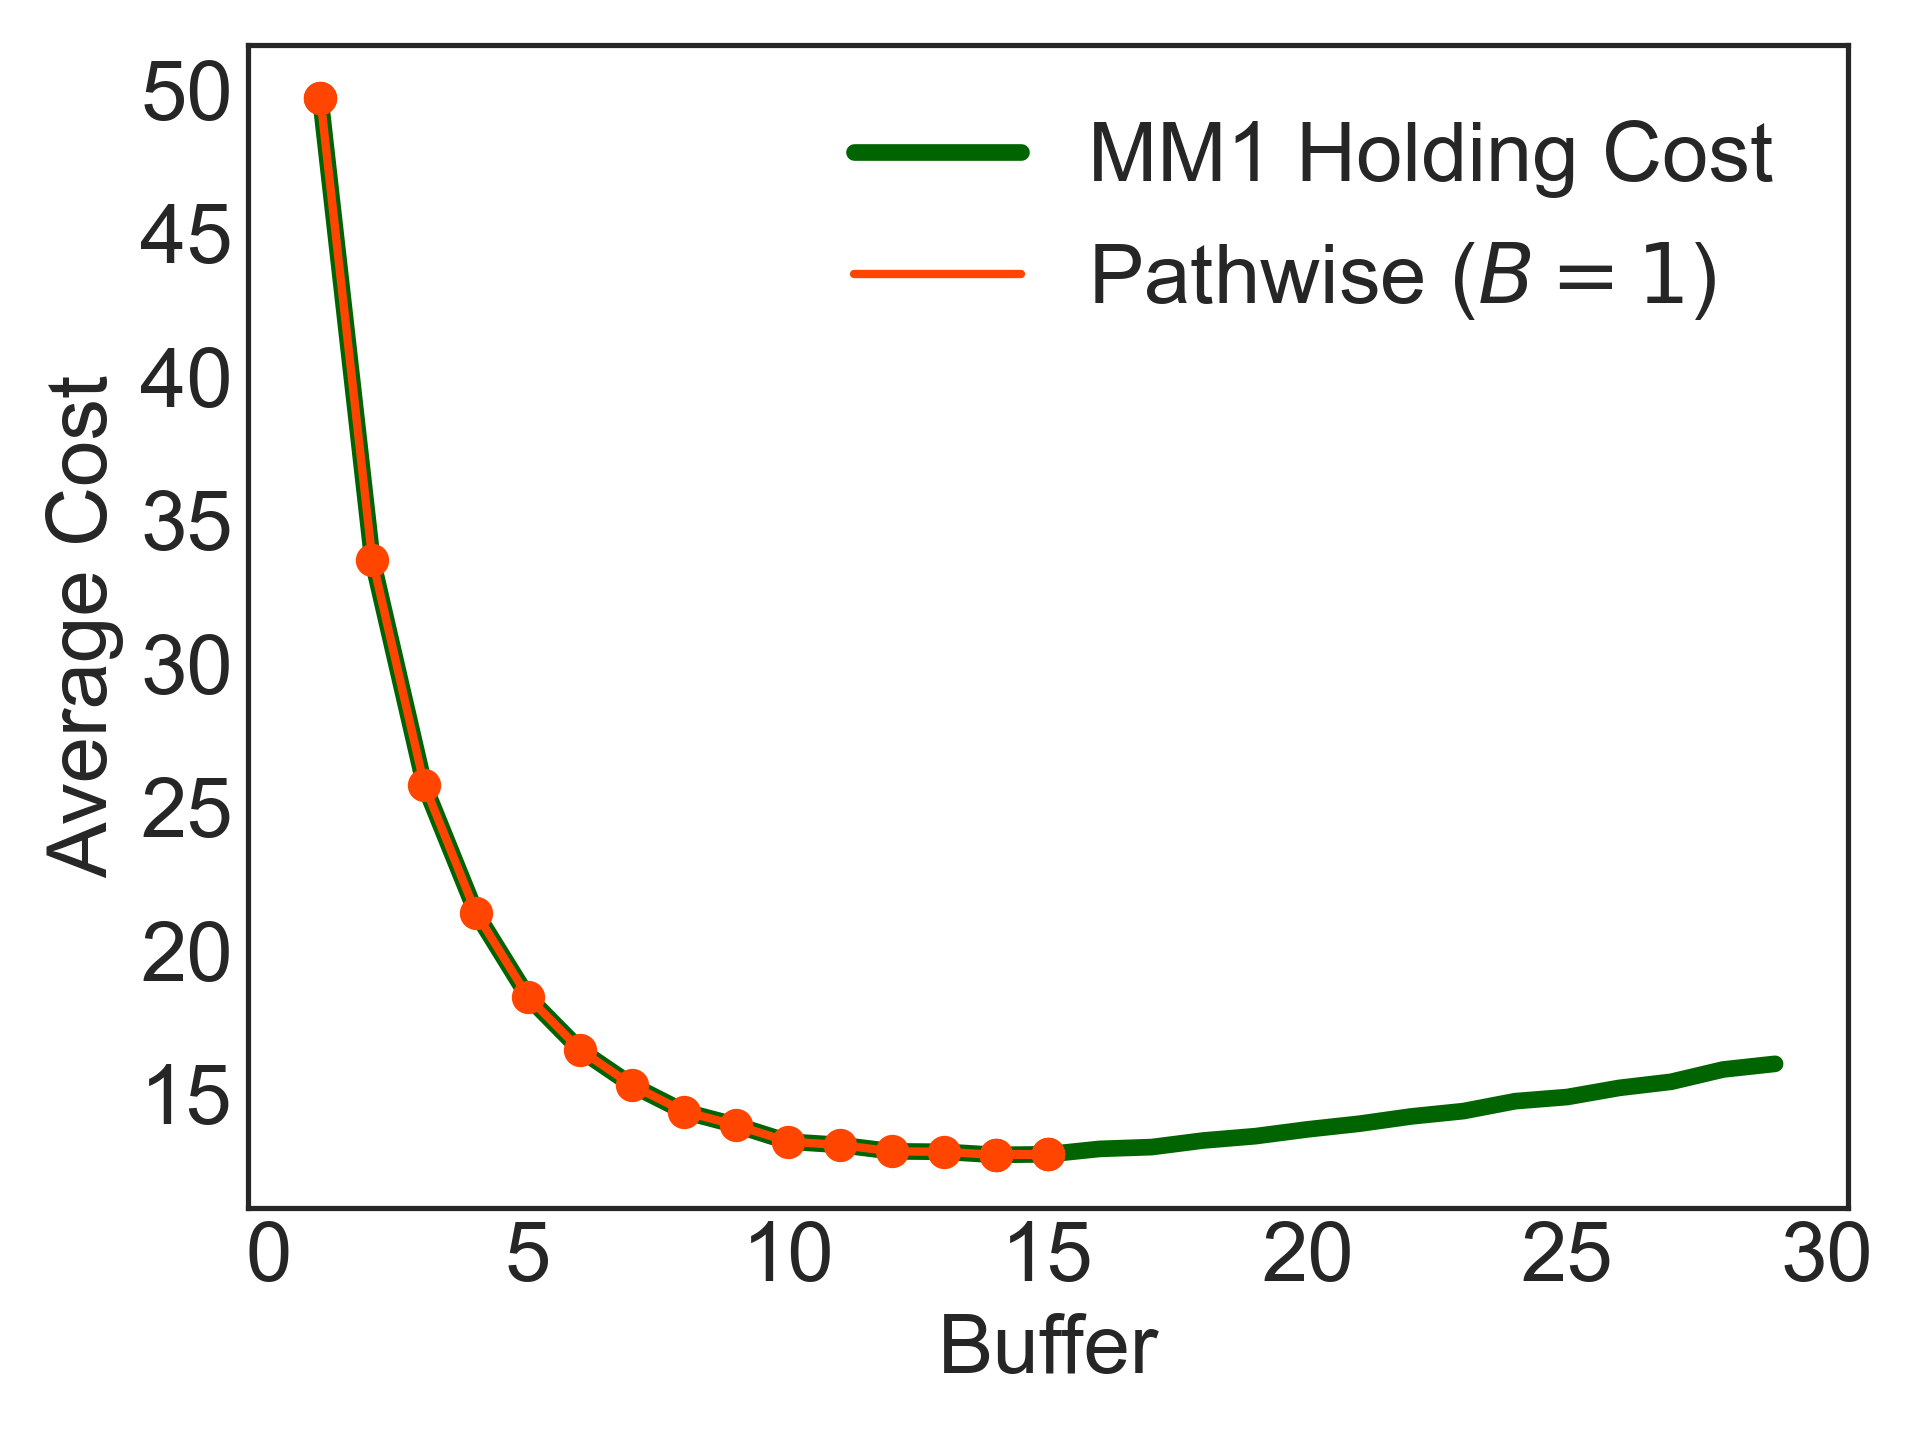
\includegraphics[height = 2.3in]{plot/gradient_eval/mm1_buffer_control_sgn.png}
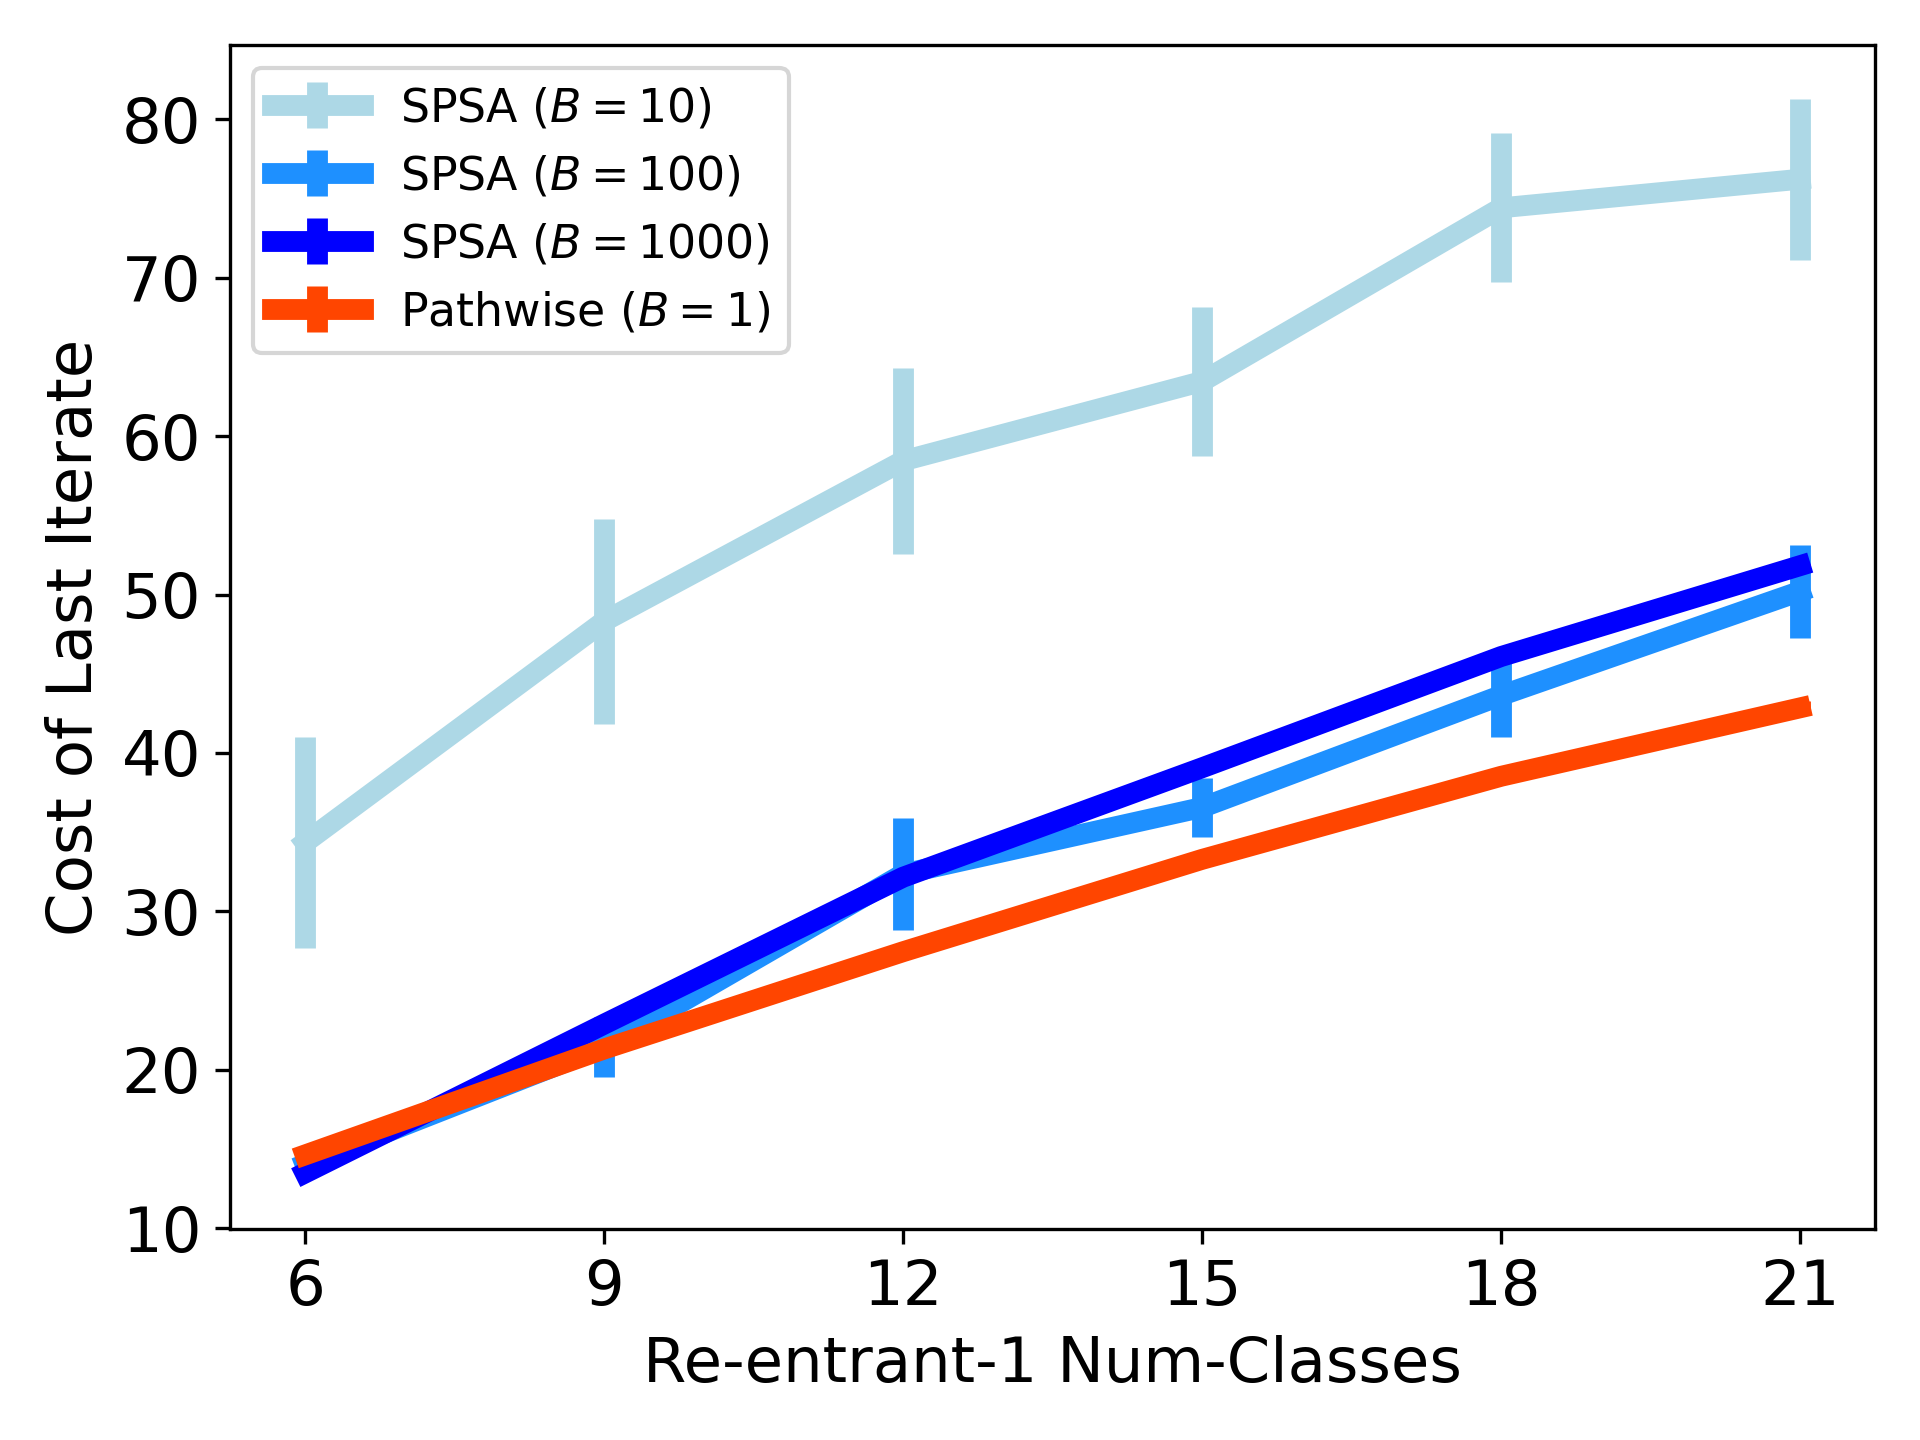
\includegraphics[height = 2.3in]{plot/gradient_eval/reentrant_1_buffer_control_1.png}
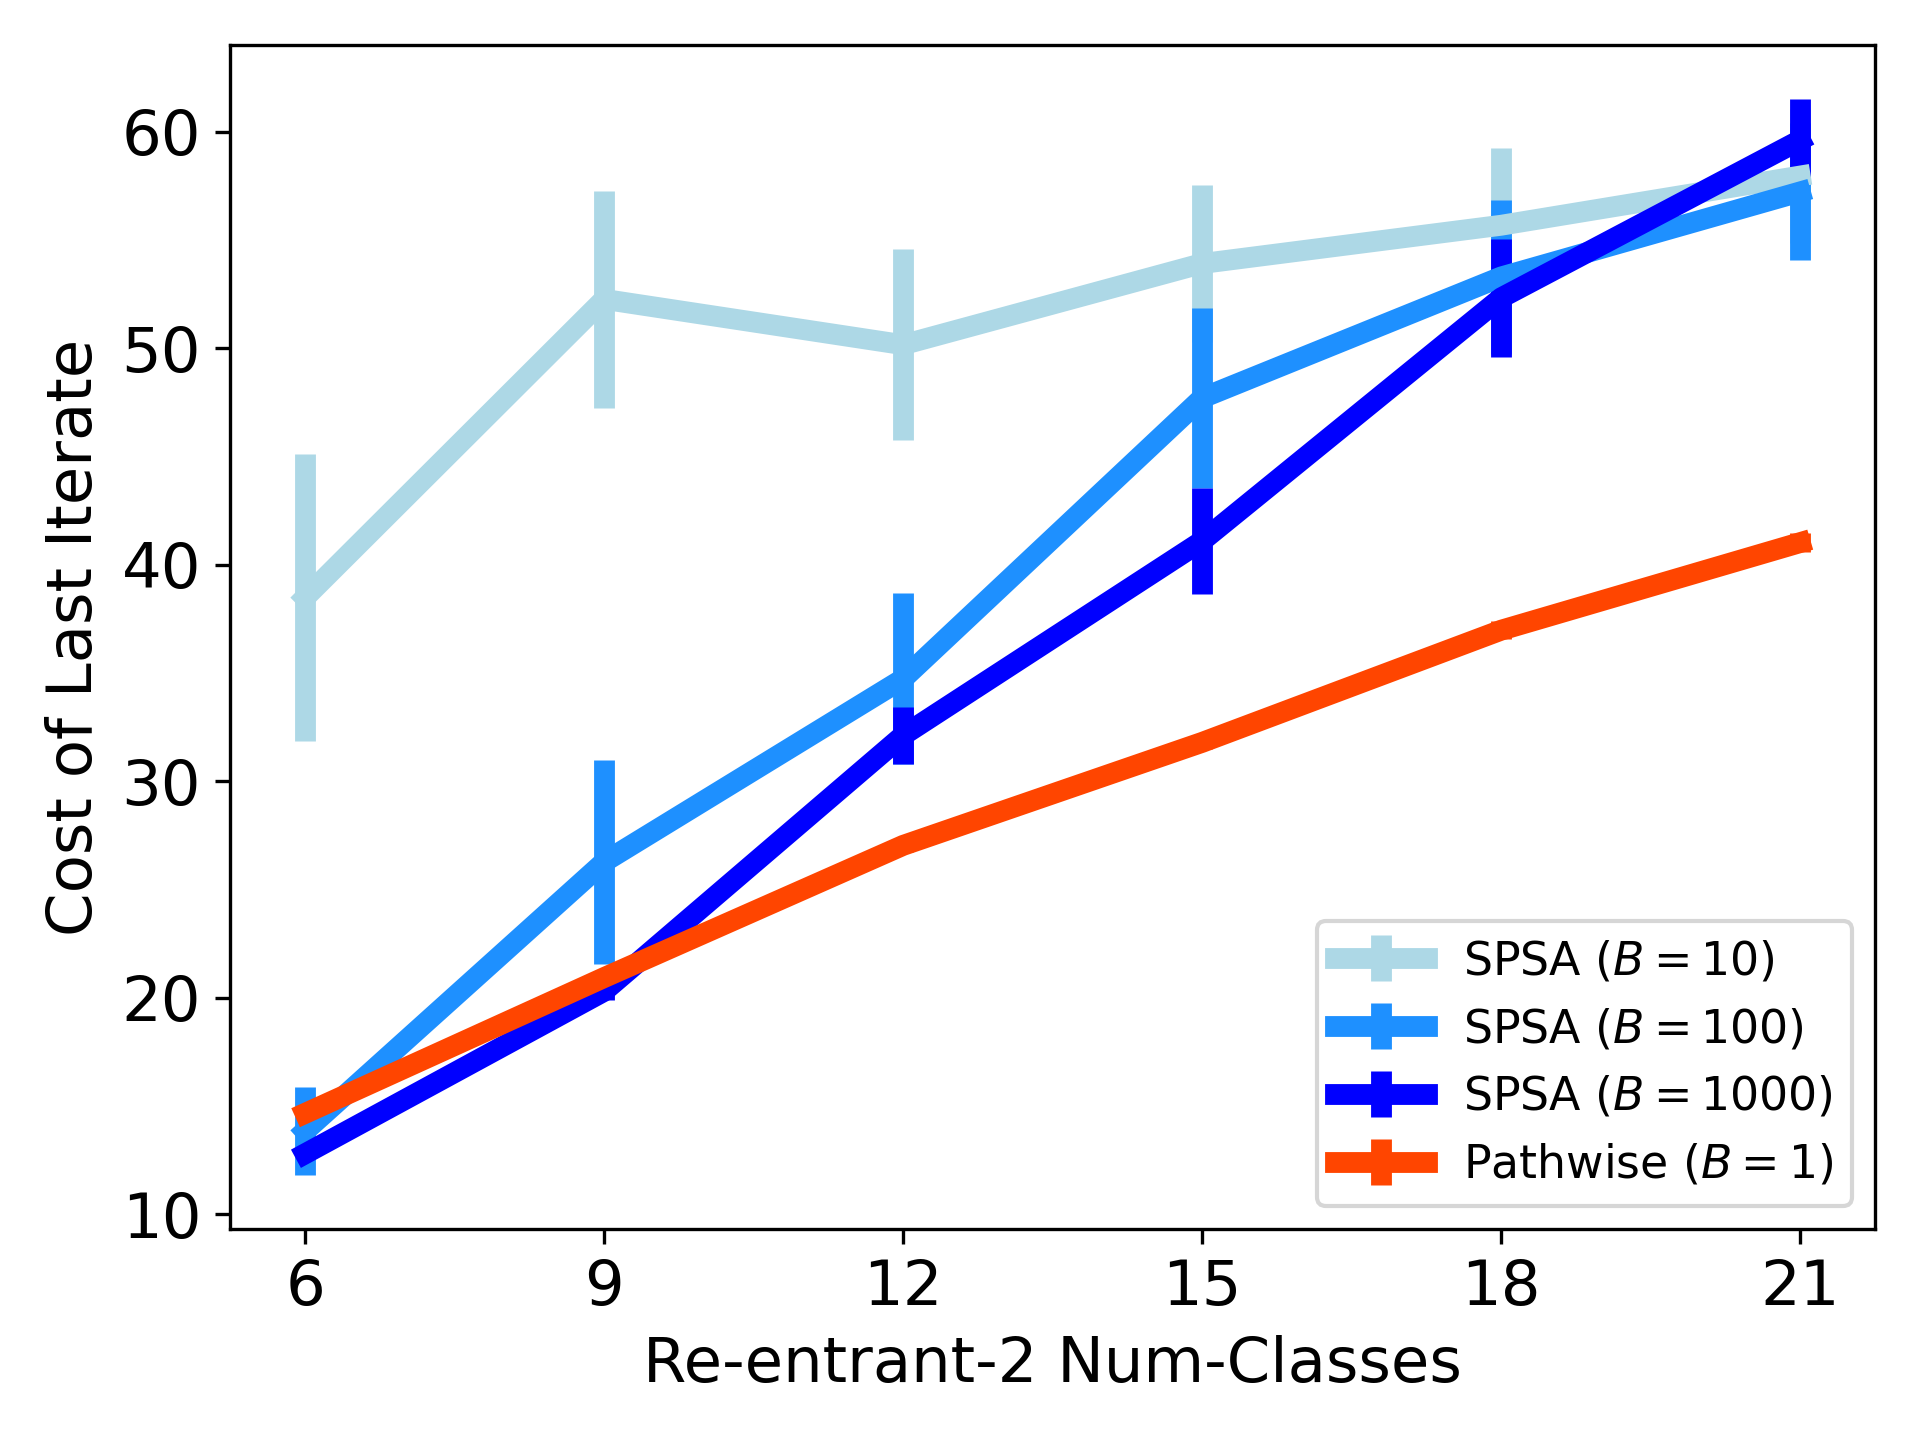
\includegraphics[height = 2.3in]{plot/gradient_eval/reentrant_2_buffer_control_1.png}
    
\caption{Last iterate performance of $\pathwise$ ($\beta = 1$) and SPSA~\cite{spall1992multivariate} on admission control for re-entrant networks. (Left) Average cost of the last iterate of sign gradient descent (100 iterations) for the Re-entrant 1 networks, across different numbers of job classes. While SPSA averaged across $B = 100$ trajectories achieves good performance, using a smaller batch $B = 10$ leads to instabilities that lead to much higher costs. $\pathwise$ with only 1 trajectory is able to consistently achieve a smaller cost, especially for larger networks. (Right) Average cost of the last iterate of sign gradient descent (100 iterations) for the Re-entrant 2 networks. Even with $B = 1000$ trajectories, SPSA is unable to effectively optimize the buffer sizes for larger networks, reaching the same cost as SPSA with $B = 10$. This illustrates that the performance of finite-difference methods such as SPSA degrade in higher-dimensional problems, whereas $\pathwise$ performs well in these larger instances using much less data.}
    \label{fig:pathwise_spsa} 
\end{figure}

To see how the estimator performs in larger-scale problems, we consider the Re-entrant 1 and Re-entrant 2 networks introduced in Section~\ref{sec:gradient_efficiency} with varying number of job classes (i.e., varying number of layers). 
%Since the control problem involves a buffer size for each job class, larger networks involve higher-dimensional control problems. 
Figure~\ref{fig:pathwise_spsa} compares the last iterate performance of SPSA and $\pathwise$ for these two families of queuing networks with instances ranging from $6$-classes to $21$-classes. Holding costs are $h = 1$ and overflow costs are $b = 1000$ for all queues. We observe that $\pathwise$ with only a single trajectory is able to outperform SPSA with $B = 1000$ trajectories for larger networks. Sign gradient descent using SPSA with only $B = 10$ trajectories is much less stable, with several of the iterations reaching a sub-optimal set of buffer sizes that assign $L_{j} = 0$ to several queues. This illustrates the well-known fact that for high-dimensional control problems, zeroth-order methods like SPSA must sample many more trajectories to cover the policy space and their performance can scale sub-optimally in the dimension. Yet $\pathwise$, which is an approximate first-order gradient estimator, exhibits much better scalability with dimension and is able to optimize the buffer sizes with much less data.


\begin{figure}[t]
\centering
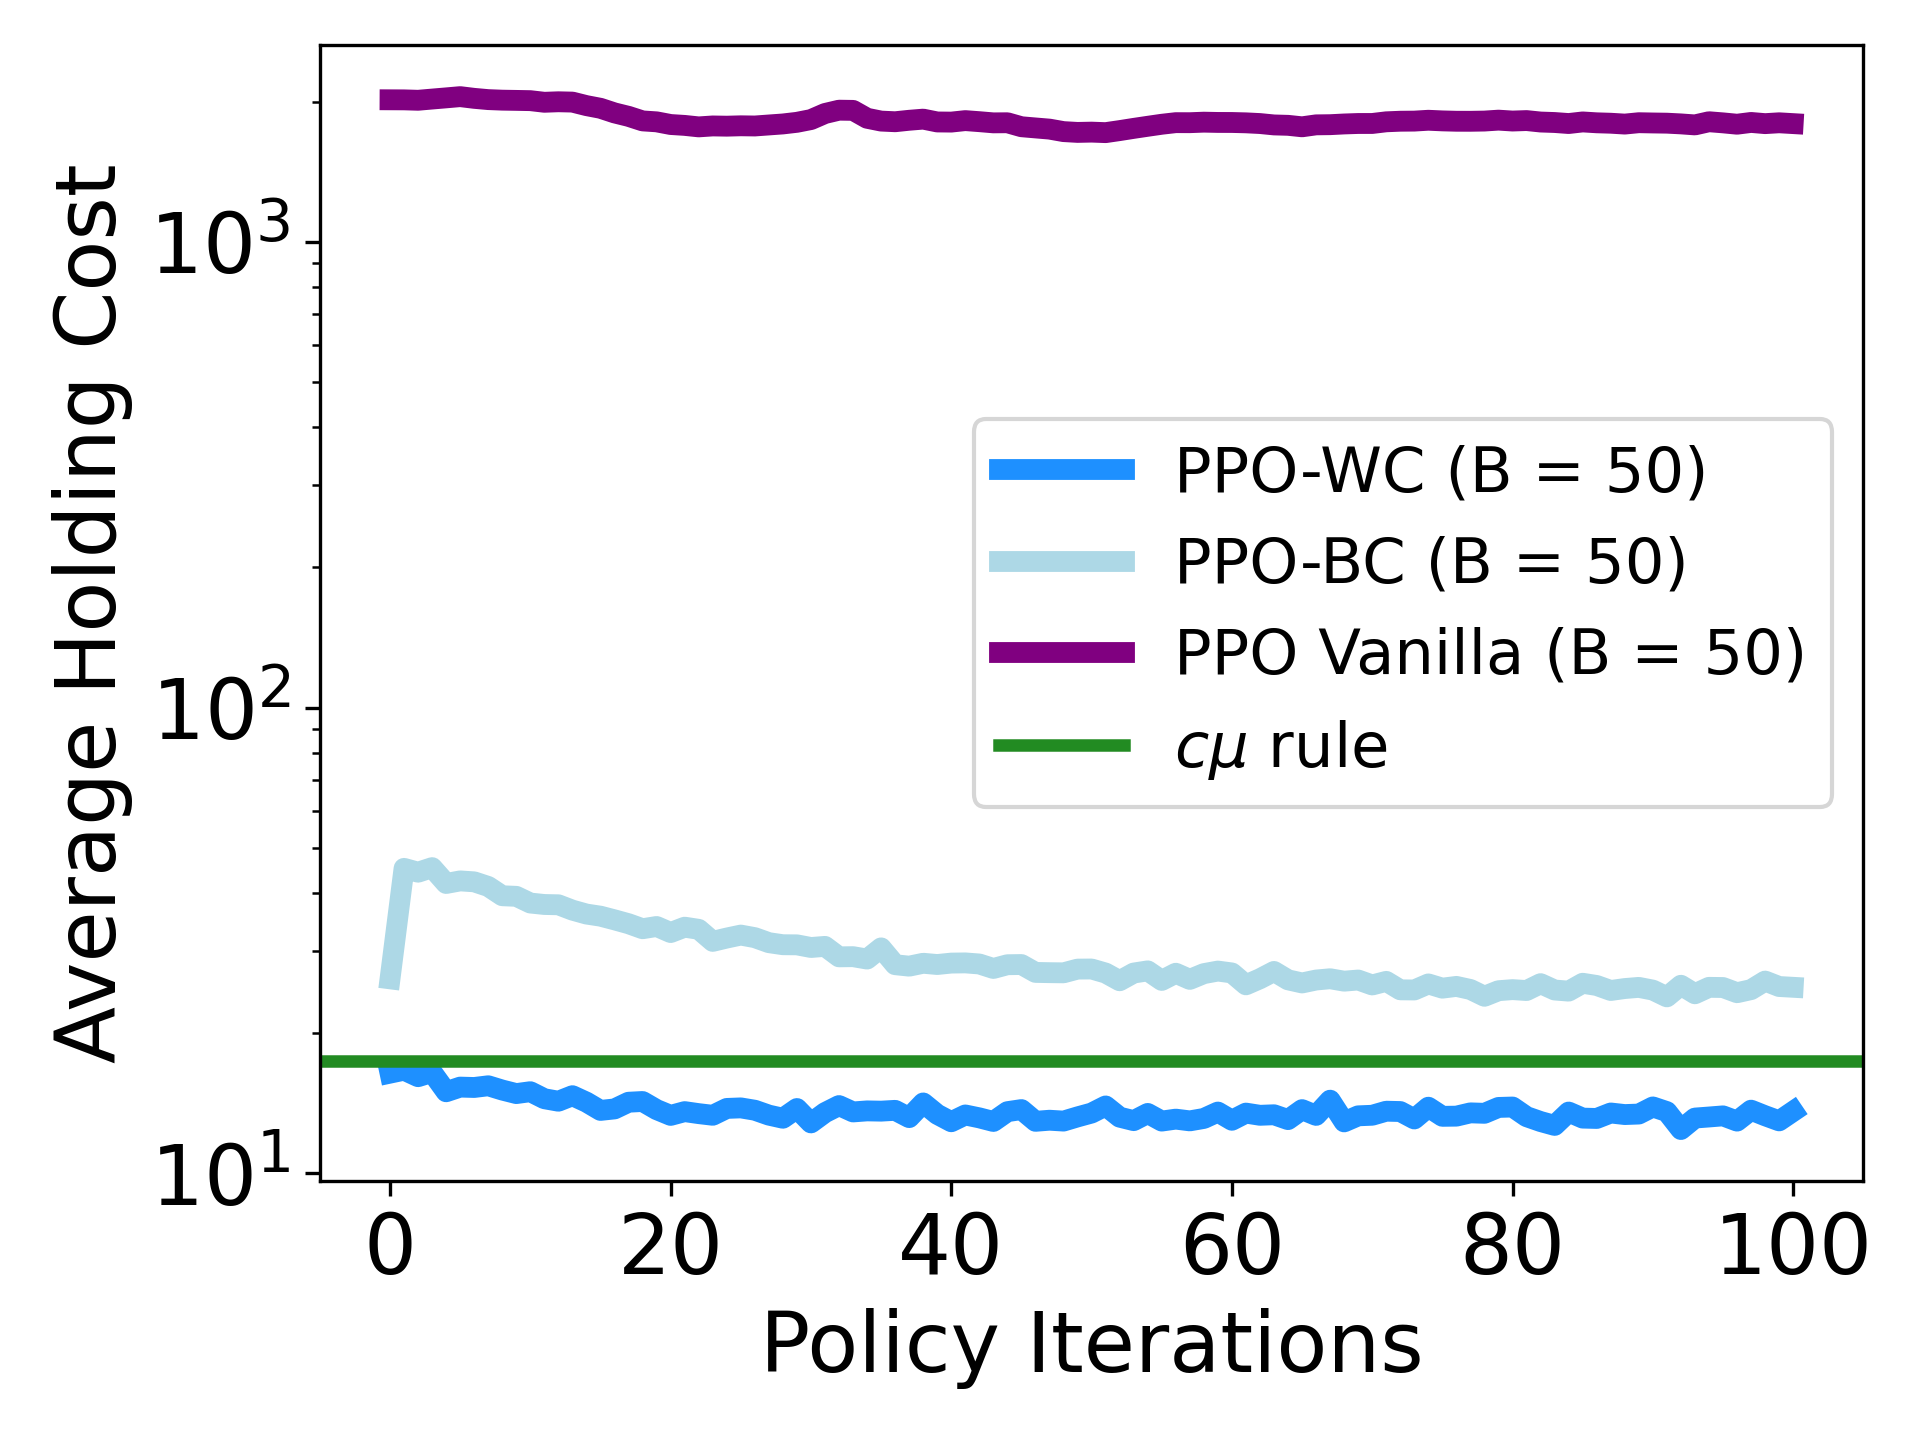
\includegraphics[height = 2.5in]{plot/policy_opt/work_conserving.png}
% 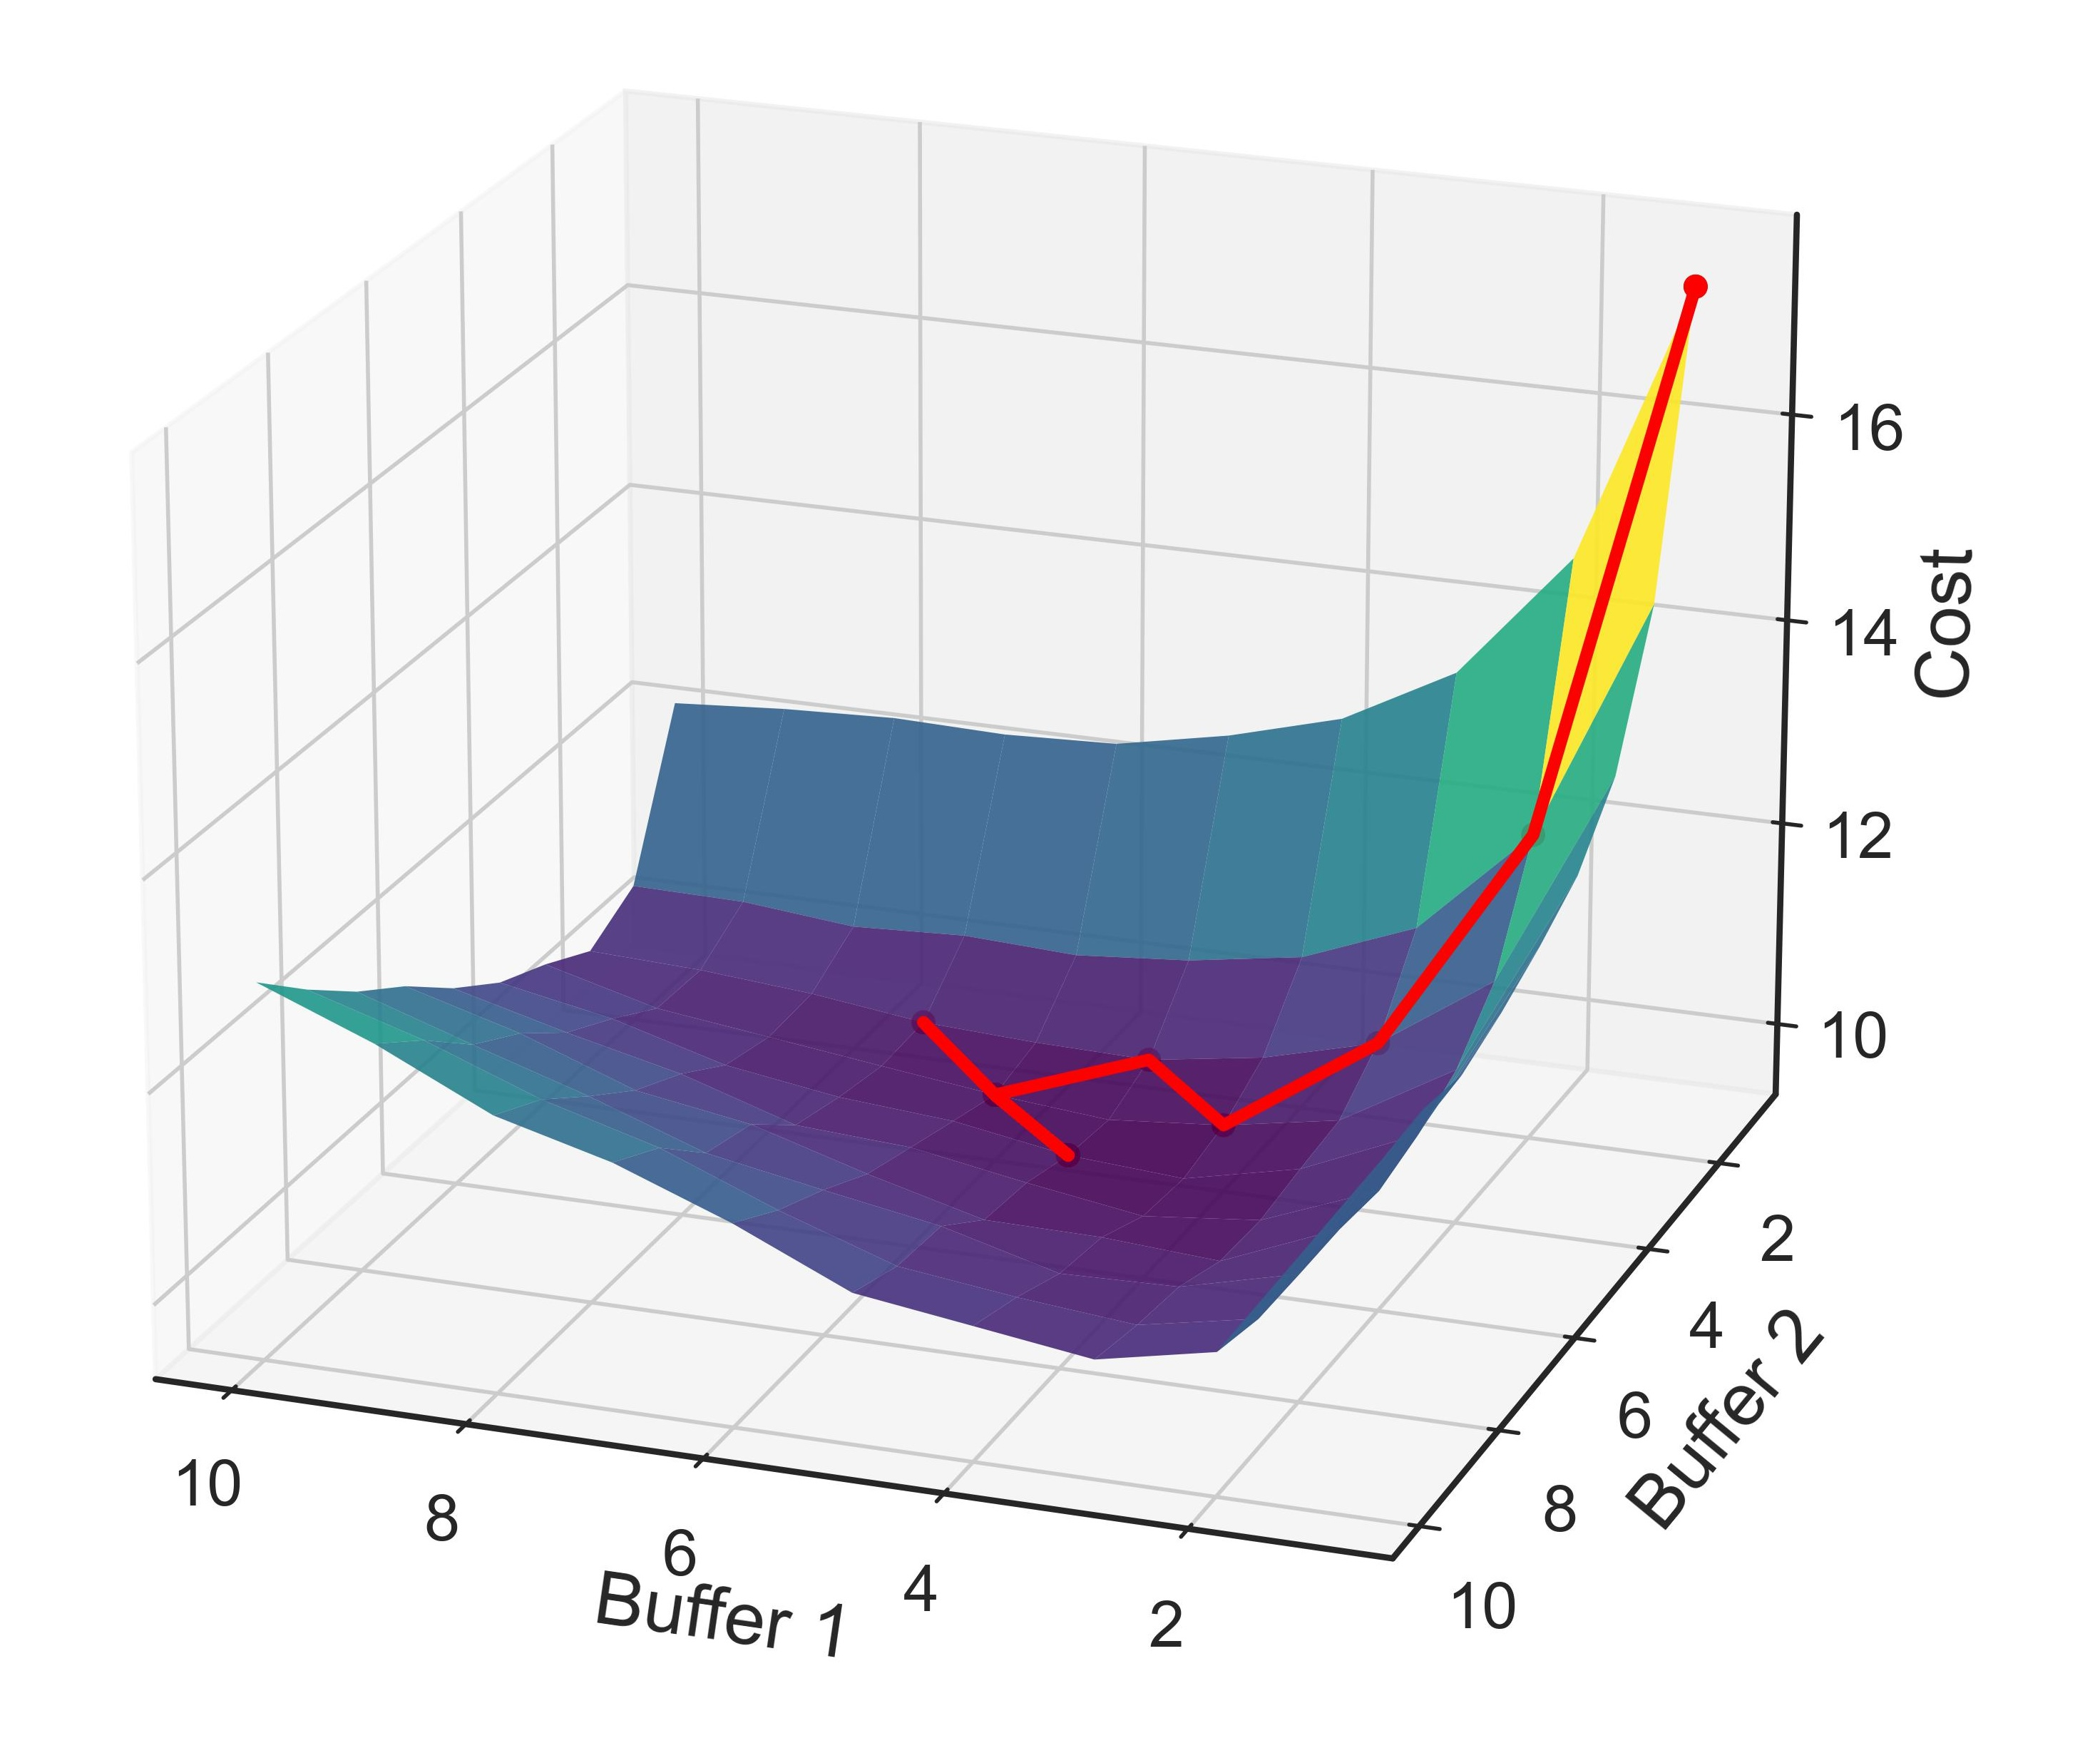
\includegraphics[height = 2.5in]{plot/gradient_eval/multiclass_admission_control.jpg}
    
    \caption{Performance of PPO with and without work-conserving softmax for the Re-entrant 1 network with 6 classes. Average holding cost of PPO without any modifications, PPO initialized from a behavior cloned policy (PPO BC), and PPO with the work-conserving softmax (PPO WC). Average cost of the $c\mu$-rule added for reference. Without any modification, PPO is unable to stabilize the queues, resulting in an average queue-length of $10^{3}$ and does not improve over time. Behavior cloning provides a much better initialization, and the policy improves with training. However, it fails to improve over the $c\mu$-rule. With the work conserving softmax, even the randomly initialized policy is capable of stabilizing the network -- achieving an equivalent cost as the $c\mu$-rule -- and is able to outperform the $c\mu$ over the course of training.}
    \label{fig:work-conserving} 
\end{figure}